\chapter{Vital sign estimation using wearable devices}

\label{chapter:PPG signal Processing} 

\section{Introduction}

Wearable devices such as wristbands and smart watches are increasingly being used to monitor the physiological parameters of individuals to track changes in heart rate, oxygen saturation and respiratory rate \cite{castaneda2018review}. Data can be acquired without imposing a disruption to a subject's daily schedule, providing a more informed assessment of the subject's well-being and helping detect health problems that might have otherwise been missed. The availability and low cost of wearables could therefore provide new ways to monitor children's health in LMICs. The aim of the chapter is to compute HR, RR and changes in $SpO_{2}$ from data recorded from a wearable device in a clinical study involving healthy volunteers undergoing a hypoxia protocol. 


\section{Data set}

The clinical study took place at the Cardiovascular Clinical Research Facility, John Radcliffe Hospital, Oxford, UK. It was a collaboration between the Institute of Biomedical Engineering and clinicians from the Nuffield Department of Clinical Neurosciences at the University of Oxford. The study received ethical approval by the East of Scotland Research Ethics Service REC 2 (19/ES/0008). The study was carried out to test the performance of wearable devices in a simulated clinical setting during hypoxia exposure (low oxygen levels).  

\subsection{Participant recruitment and assessment}

43 healthy volunteers were recruited for the study. Written consent was obtained for each study participant. The screening assessment for the study was completed by an appropriately qualified, medically trained member of the research team, who confirmed the volunteers' eligibility. Participants were excluded if incomplete data were collected for any one device during the duration of the study, or if hypoxia was not achieved.

Demographics data including age, sex, height, weight, skin type (Fitzpatrick scale \cite{gupta2019skin}), heart rate and SaO2 (from arterial blood gas (ABG)) were collected for each participant, at the start of their sessions and recorded in a Case Report Form (CRF). All data from participants were identified using a study number. Four participants presented adverse clinical conditions (three anaemia cases - evaluated from the first ABG - and one sickle cell trait). Therefore, 39 complete data sets were acquired in total. The summary of the demographic information of the study volunteers is presented in table ~\ref{table:demographics}. 

%
%
% Mauro: [hbt]
% Mauro: [!hbt]
\begin{table}
	\centering
	\caption{Summary of the population in the clinical study.}
	  {\small
	   \singleTableRowHeight
	   \begin{tabular}{ll}
	     \tableHeaderStart
	        \tableHCell{Description} & \tableHCell{Value} \\
	     \tableHeaderEnd
	     Total number of complete recording sessions   & 39 \\
	     Average length of a recording session (minutes) & 18.4  \pm{} 2.9 \textsuperscript{1}  \\
	    \textbf{Gender}          &        \\
	    \hspace{3mm}Females      & 21 (53.8\%)\textsuperscript{2}  \\
	     \hspace{3mm}Male            & 18 (46.2\%)\textsuperscript{2}  \\
	    Age   & 32.6 \pm 10.4\textsuperscript{1}  \\  
	    Weight                 & 71.2 \pm 13.4\textsuperscript{1}               \\
	    Height(m) & 1.71 \pm 0.10\textsuperscript{1}  \\                 
	\textbf{Fitzpatrick Skin type} &  \\
	 \hspace{4mm}Type I & 10 (25.6 \%)\textsuperscript{2}     \\
	 \hspace{4mm}Type II & 18 (46.2 \%)\textsuperscript{2}    \\
	 \hspace{4mm}Type III & 2 (5.1 \%)\textsuperscript{2}        \\
	 \hspace{4mm}Type IV & 9 (23.1 \%)\textsuperscript{2}      \\  
	\hline    
	      \multicolumn{2}{l}
	      {
	\footnotesize $^1$ mean \pm{} standard deviation
	      } \\
	 \multicolumn{2}{l}
	 {
	\footnotesize$^2$ Total number (percentage)
	  }\\
	     \end{tabular}
     }
	\label{table:demographics}
\end{table}

\subsection{Study set-up}

The study participants lied comfortably on a bed  in a semi-horizontal, supine position. A tight-fitting silicone face mask was placed and connected to a hypoxicator unit (Everest Summit Hypoxic Generator). If required, additional 7\% oxygen in nitrogen from a cylinder was added into the hypoxicator circuit to ensure tight control of fraction of inspired oxygen (FiO2) provided to the participant. SaO2 readings were taken for the 100\%, 95\%, 90\%, 87\%, 85\%, 83\% and 80\% SpO2 target values, with the corresponding output of the blood gas analyser then taken as the reference value. 
$SpO_{2}$ stability was subjective for each target SaO2 window, i.e. a senior
anaesthetist decided when a stable oxygen level was achieved in order to take the ABG, based on the clinical values shown by the standard $SpO_{2}$ monitor. $SpO_{2}$ measurements of greater than or equal to 90\% were considered normoxia, while levels between 85\% and 89\% were considered mild hypoxia. Oxygen saturation levels below 85\% were regarded as severe hypoxia.

\subsection{Instrumentation}

Participants wore several ambulatory monitoring devices (AMD) including a purely wrist worn device (Wavelet Health, USA) and up to three wrist-worn devices with finger probes. In this chapter, data from the Wavelet wristband, wearable device using reflectance PPG to measure pulse rate was used. The device records 1 minute red and near-infrared (NIR) time series data with 1 minute gaps in between at a sampling rate of 79Hz. Other sensors in the Wavelet Health include 3-axis accelerometer sensor (recorded at 10Hz) and gyroscope.

The Philips Monitor MX450 was used as the reference clinical standard device, recording \gls{$SpO_{2}$} values and HR at a sample rate of 1Hz. Figure ~\ref{physio} shows a 30-minute window of vital signs measured using the Philips monitor, as well as the red/NIR signals recorded from the Wavelet Health device. 

\begin{figure}
	\centering
	 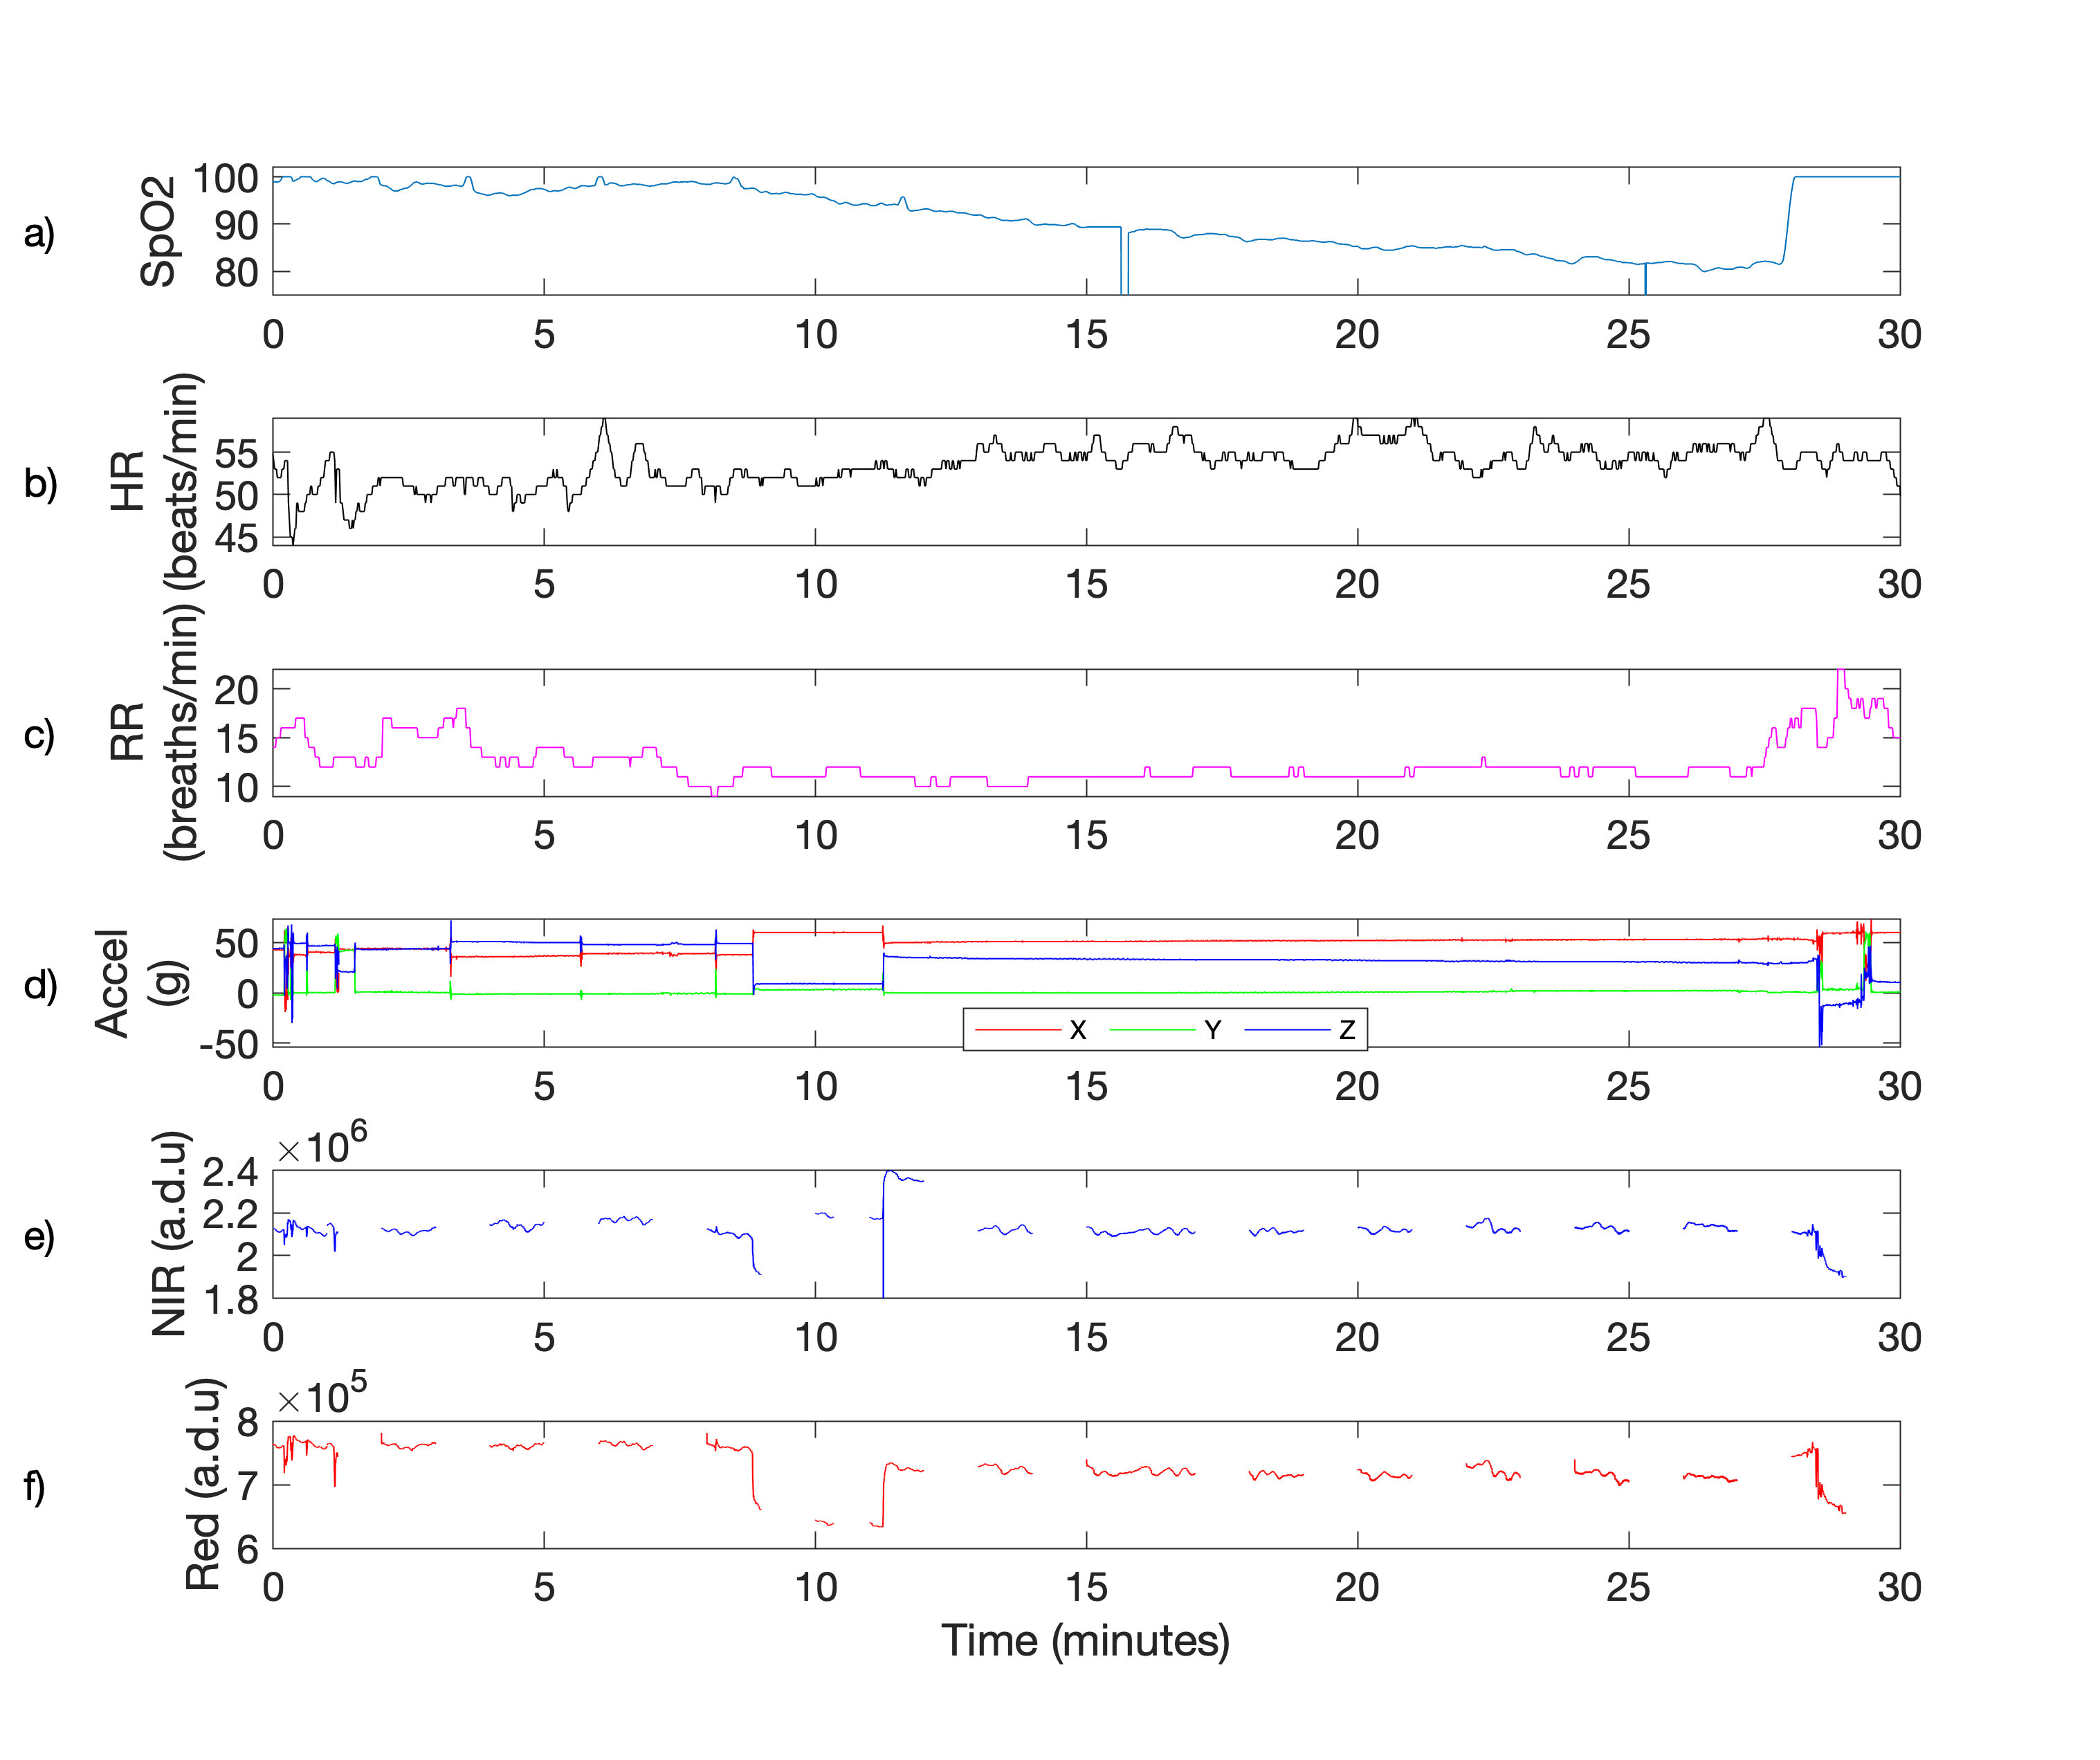
\includegraphics[width=0.8\linewidth,keepaspectratio=true]{Comparefigure}
	    \caption[Reference physiological parameters recorded by the Phillips monitor and the Wavelet Health device.]
	    {
	    Physiological parameters recorded by the Phillips monitor and the Wavelet Health device. 
	    a) \gls{$SpO_{2}$} from the Phillips monitor. Lowest recorded Oxygen saturation was 80\% as per protocol. b) Heart rate and c) Respiratory rate from the Philips monitor. d) Accelerometer data recorded by Wavelet Health. e) Raw NIR signal and f) Red signal from the Wavelet Health device. The device records 1 minute data on and off.\\
	    }      
	 \label{physio}  
\end{figure}

\subsection{Data selection}
39 complete data sets were acquired. 28 sessions with data that was greater than 20 minutes in length were selected; to allow 2 minutes for recovery to normal oxygen saturation (>90\%) . 19 sessions were subsequently selected because these data sets were not corrupted by motion. Finally 10 sessions were selected for analysis in this report. Figure ~\ref{selection} shows a summary of the data collection criteria.

\begin{figure}
    \centering
\includegraphics[width = 12 cm]{nicu_selection}
    \caption{Flow diagram outlining the patient selection process.}
    \label{selection} 
\end{figure}

Figure ~\ref{vs hist} shows the distribution of HR, $SpO_{2}$  and RR values from the 10 chosen volunteers. Mean $SpO_{2}$  = 91.2\%, Median $SpO_{2}$ = 90.9\%, Inter-quartile range = 13.9. The mean HR was 66.3 beats/minutes. Median HR = 65 beats/minutes, inter-quartile range = 12. Mean RR = 14.1 breaths/minutes, Median RR = 14 breaths/minutes, Inter-quartile range = 55.

\begin{figure}
    \centering
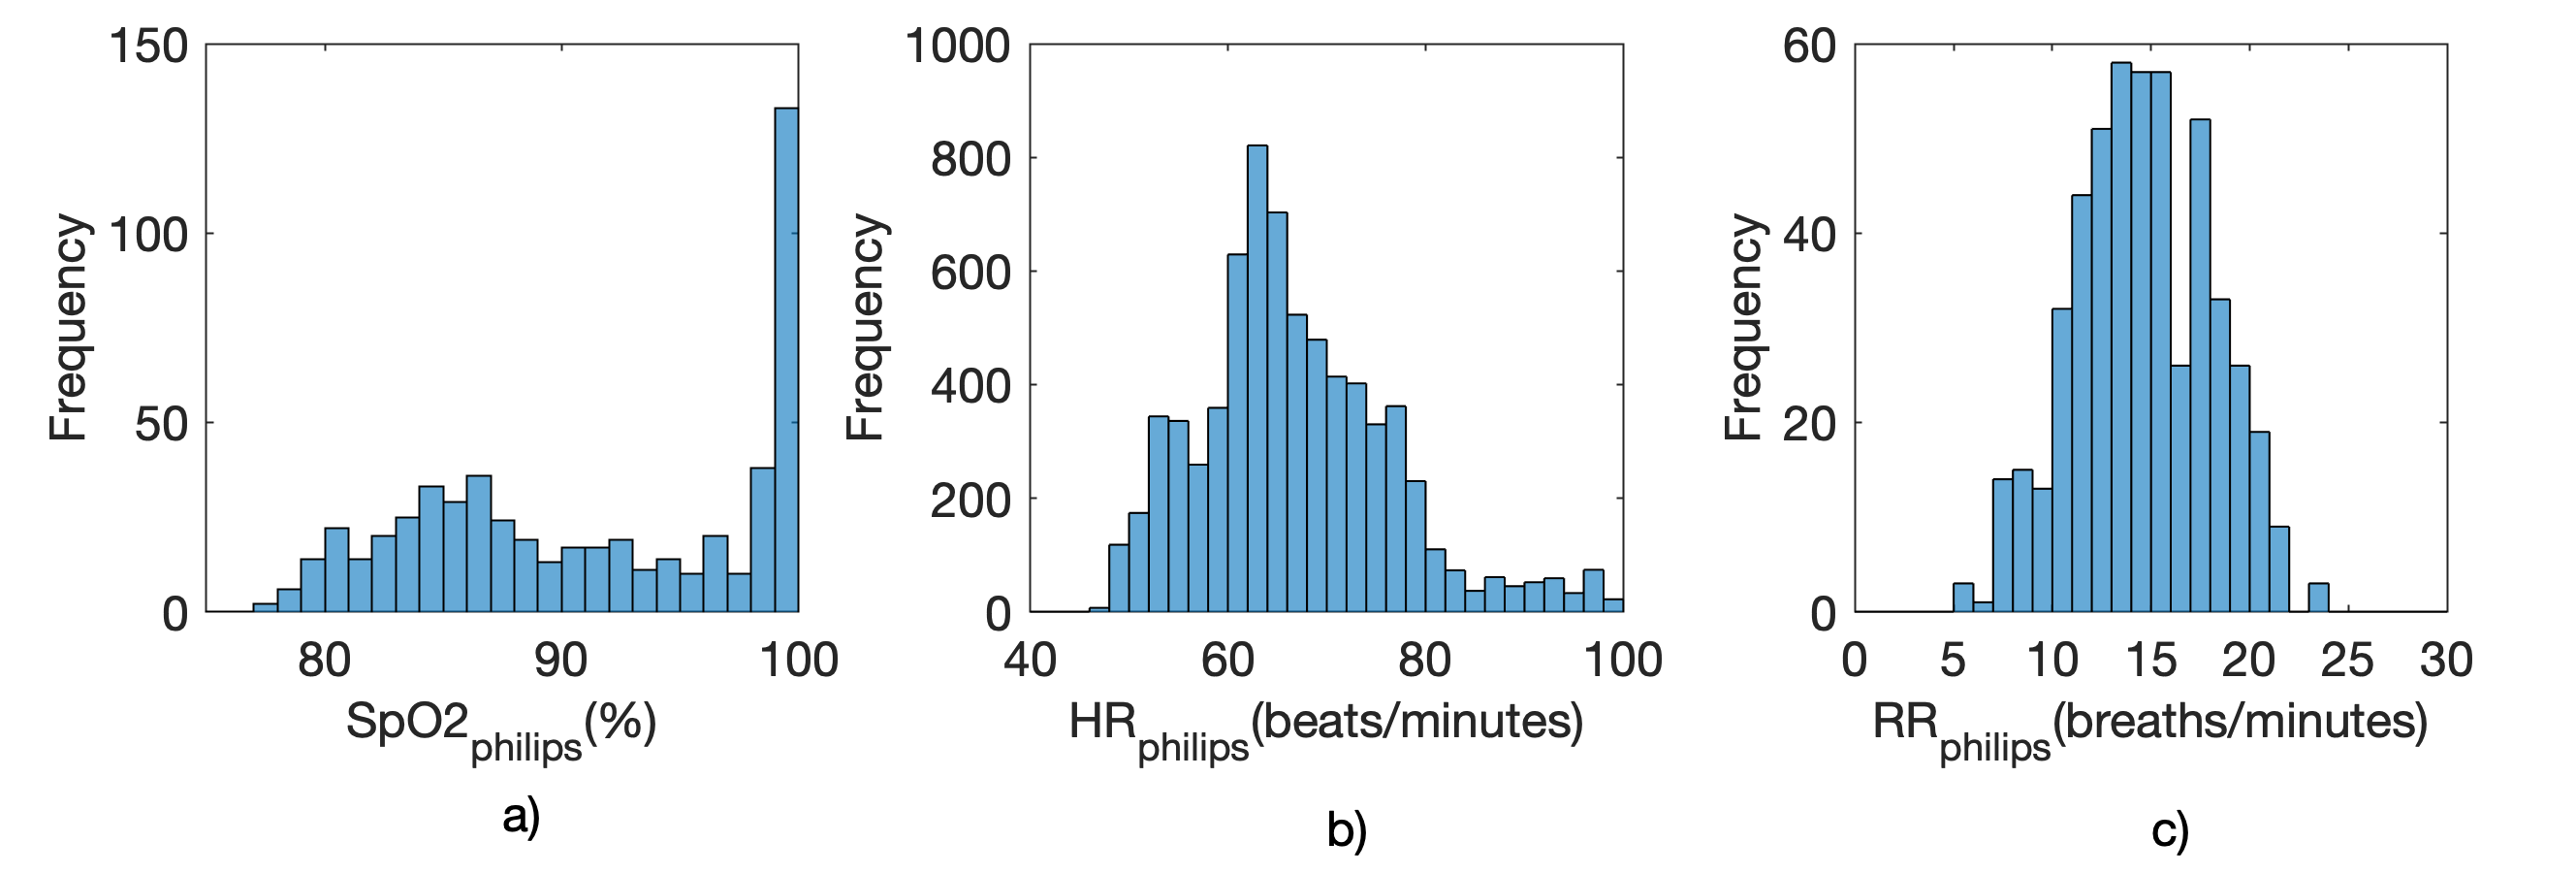
\includegraphics[width = 12 cm]{Overall_Histogram_plot}
    \caption [Distribution of vital signs recorded by the Philips monitor for the 10 sessions selected for analysis.]{Distribution of vital signs recorded by the Philips monitor for the 10 sessions selected for analysis. a)$SpO_{2}$; b) HR and c) RR}. 
    \label{vs hist} 
\end{figure}

\section{Heart rate estimation}
\label{HR est_wav}


\subsection{Overview of the process}

HR is used frequently in healthcare and easily extractable from a PPG signal, as pulsatile blood flow from the heart modifies the absorption of NIR light. The NIR signal was detrended and filtered to remove noise. The filtered signal was then split into 10s windows, and the peaks of the pusatile signal were detected for each of these windows. These peaks were counted to estimate HR. A motion SQI was then applied using accelerometer data from the Wavelet Health device, which discarded HR estimates where the NIR signal was corrupted by motion. Figure~\ref{HRoverview} presents an overview of the process of estimating HR using the Wavelet Health device. 

\begin{figure}
    \centering
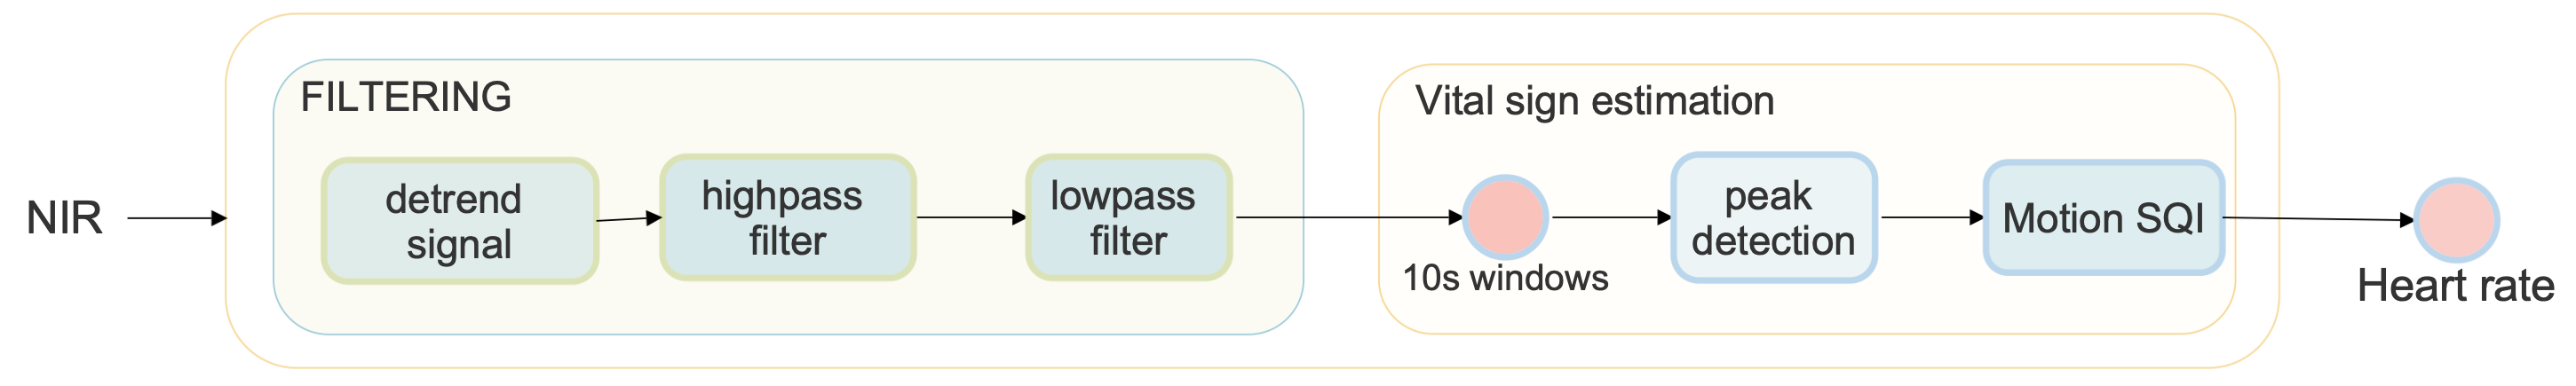
\includegraphics[width = 12 cm]{nicu_HRflowchart.png}
    \caption{Flow diagram outlining the process of computing heart rate from the NIR signal from the Wavelet Health device.}
    \label{HRoverview} 
\end{figure}

\subsection{Filtering}

The NIR signal was first detrended to remove the DC component. The de-trended signal was further processed by designing two zero-phase FIR filters, shown in figure~\ref{mag_HR}, to remove low and high frequency noise from the signal respectively. A $181_{st}$ order high-pass filter was designed with a passband frequency of  0.7Hz (42 beats/min) and a stop-band frequency of 0.3Hz (18 beats/min). A $36_{th}$ order low-pass filter was subsequently applied with a passband frequency of 2Hz (120 beats/min) and a stop-band frequency of 4Hz (240 beats/min). Both filters were designed with a passband ripple of 1dB and stop band attenuation of 20dB.
 

\begin{figure}
\centering
\includegraphics[width = 10 cm]{mag_responsehr.png}
    \caption[Magnitude responses.]{Magnitude responses for a) High-pass filter b) low-pass filter.}
        \label{mag_HR}
\end{figure}

Figure ~\ref{figfilt} shows an example plot of the NIR signal before and after de-trending and filtering. The Fast Fourier Transform (FFT) plots shown in figure~\ref{figfilt}c and figure~\ref{figfilt}d show a clear peak at 0.9 Hz corresponding to a HR of approximately 54 beats/minute. The reference HR recorded by the Philips monitor was 55 beats/minute.


\begin{figure}
\centering
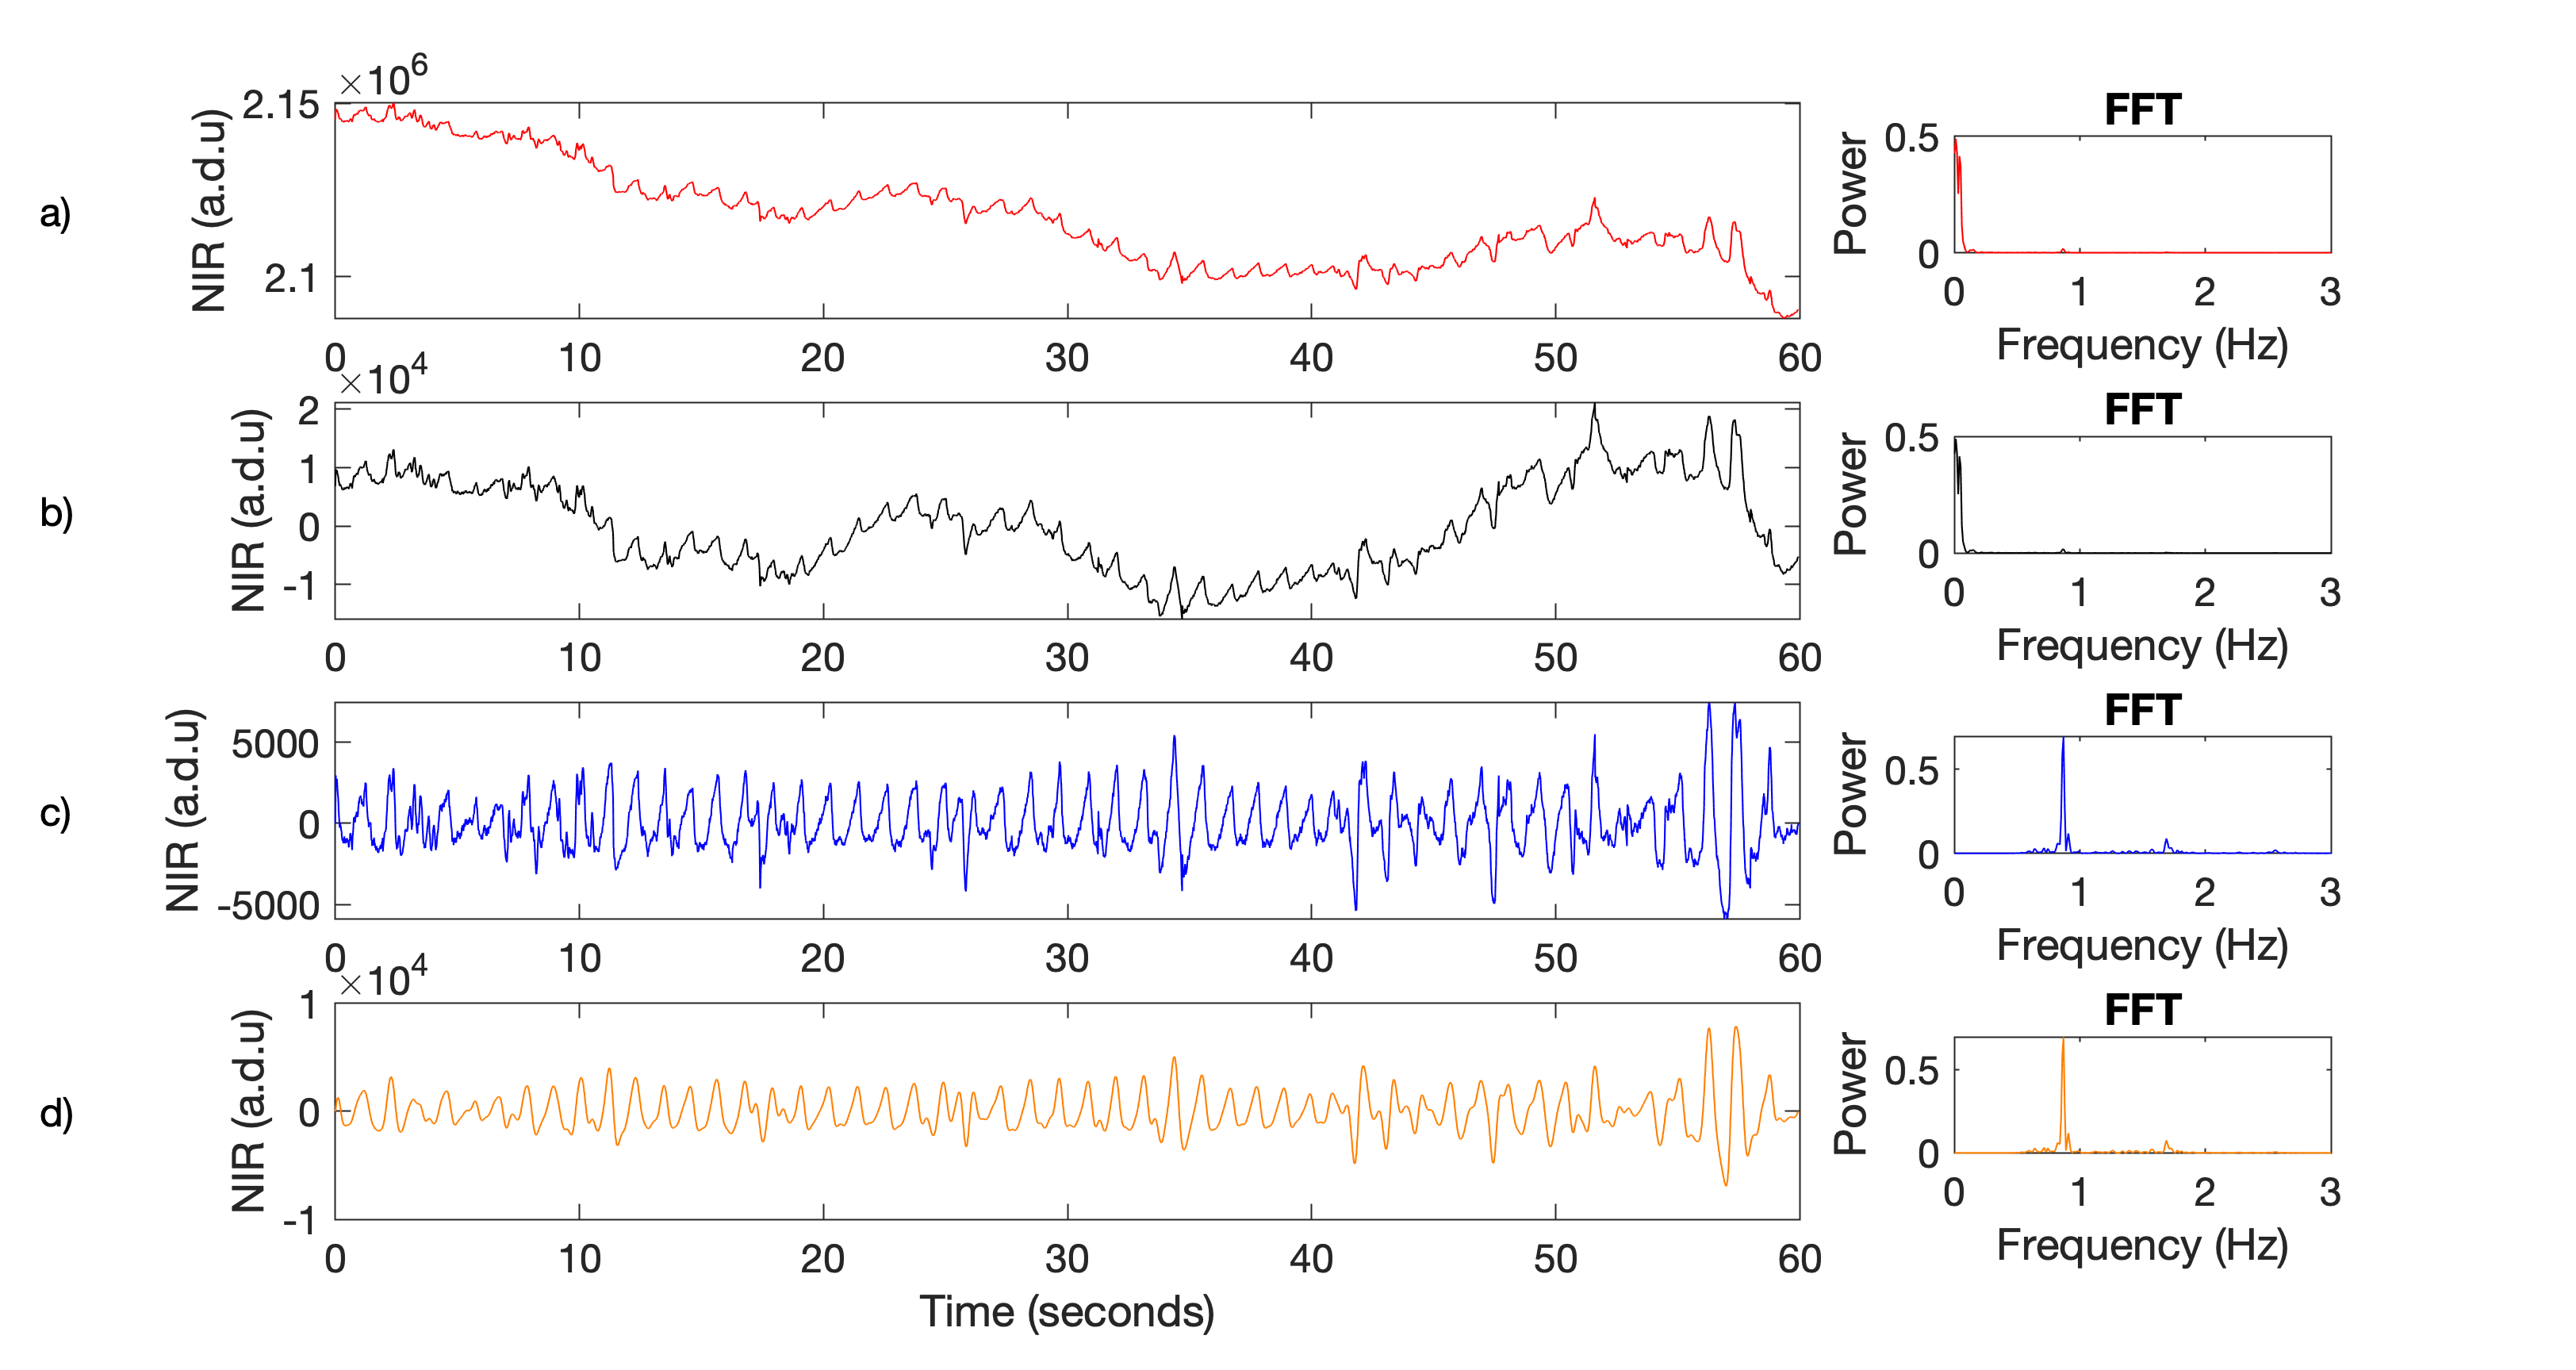
\includegraphics[width = 13 cm]{lp_filtered.png}
    \caption[60-second sample time series from the NIR waveform.]{60-second sample time series from the NIR waveform. a) Input signal; b) de-trended. Signal after the c) high-pass and d) low-pass filter were applied. The FFT panels show a peak at 0.9Hz corresponding to a HR of approximately 54 beats/minute. The reference HR recorded by the Philips monitor was 55 beats/minute.}
    \label{figfilt}
\end{figure}

\subsection{Peak detection}
\label{peak_eqn}

Peak-to-trough analysis was performed on the filtered signal. This process identified prominent maximum and minimum points in the signal to measure changes in signal amplitude. The algorithm used for peak detection first identified a peak as the $i _{th}$ sample in a time series $ts$ if: 

\begin{equation}
	ts(i) > ts(i-1)\textrm{ \textbf{and} } ts(i) > ts(i+1)
\end{equation}
To avoid reporting erroneous peaks due to noise, identified peaks were kept if:

\begin{equation}
	ts(i_{peak})  > MinPeakHeight
\end{equation}

where MinPeakHeight was set to a signal intensity of 100, based on manually observing the minimum height of waveform peaks in low intensity segments of the recording. Remaining peaks were retained if:

\begin{equation}
	i_{peak_{n}} - i_{peak_{n-1}}  >  MinPeakDistance
\end{equation}

where MinPeakDistance was set to give a refractory period (a recovery time after each peak) of 40 samples (corresponding to 84 beats/minute) based on the histogram of reference vital-sign data for the session in figure~\ref{vs hist}. Finally, peaks were selected as:

\begin{equation}
	prom(i_{peak}) > MinPeakProminence
\end{equation}

where $prom$ was the prominence of a peak, defined as the height of the peak relative to neighbouring troughs. Here, MinPeakProminence was set to a value of 58 based on manually observing peak prominences in several example recording segments. The algorithm then returned a vector containing the location and magnitude of each peak as shown in figure~\ref{peak}.

\begin{figure}
\centering
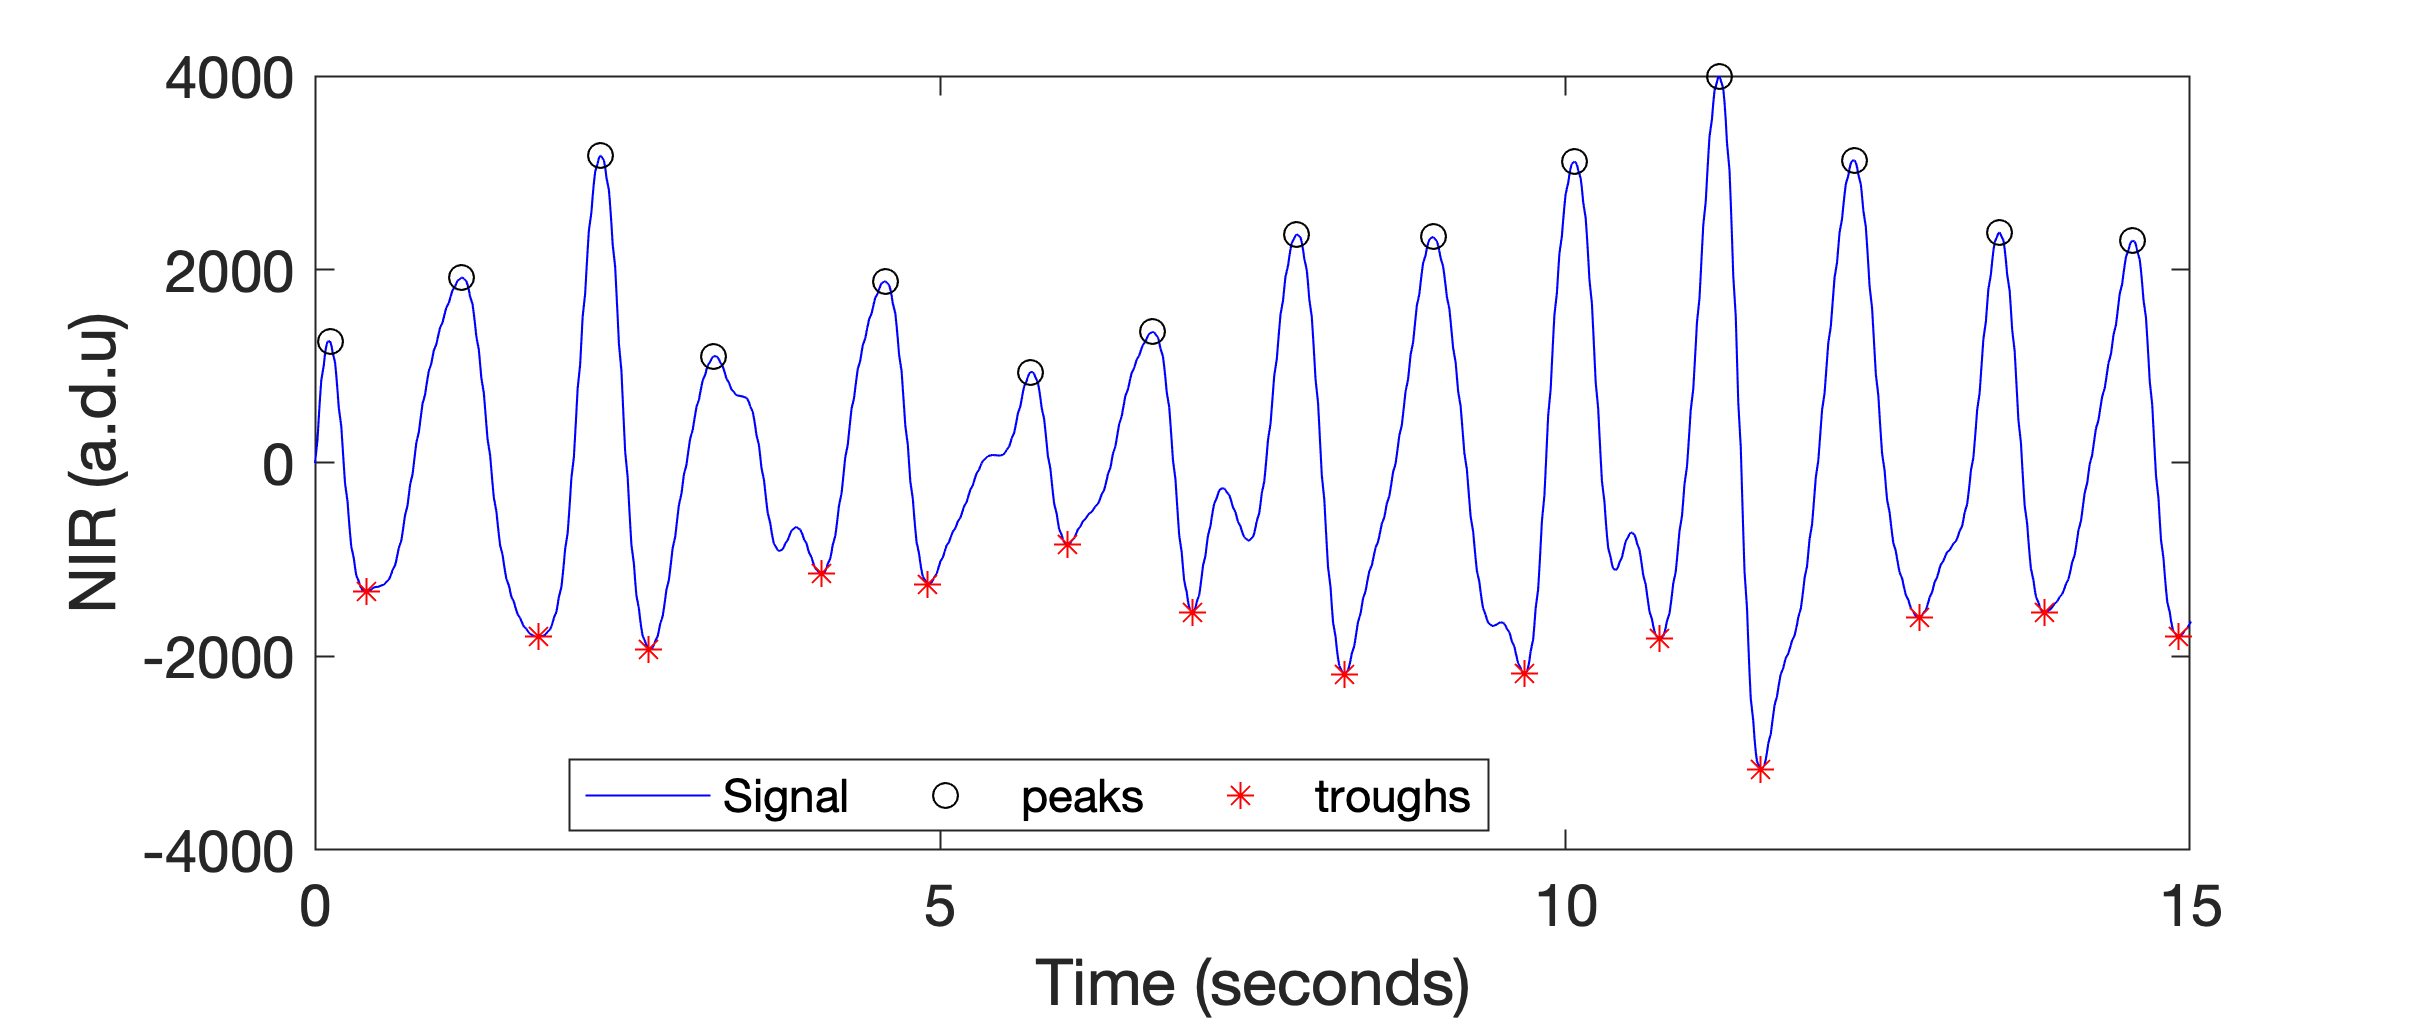
\includegraphics[width = 10 cm]{./figures/peakdetector.png}
    \caption{Detection of peaks and troughs on the NIR signal over a 15-second sample window.}
  \label{peak}
\end{figure}

\subsection{Motion SQI}

Motion analysis was used to compute a signal quality index (SQI) designed to exclude time periods during which significant movement artefacts occurred. The accelerometer data recorded by the Wavelet health device was first split into 5-minute non-overlapping windows. Subsequently, the mean and standard deviation were calculated for each window. Data points for which the acceleration was greater than \pm{}2 standard deviations from the mean for that window were considered to have an SQI of 0, corresponding to time periods of motion; otherwise an SQI of 1 was assigned, corresponding to time periods of good quality. Finally, the NIR signal within \pm{}3 s of any accelerometer data with an SQI of 0 were discarded. An example of this process is shown in figure~\ref{SQIACC}.


\begin{figure}
\centering
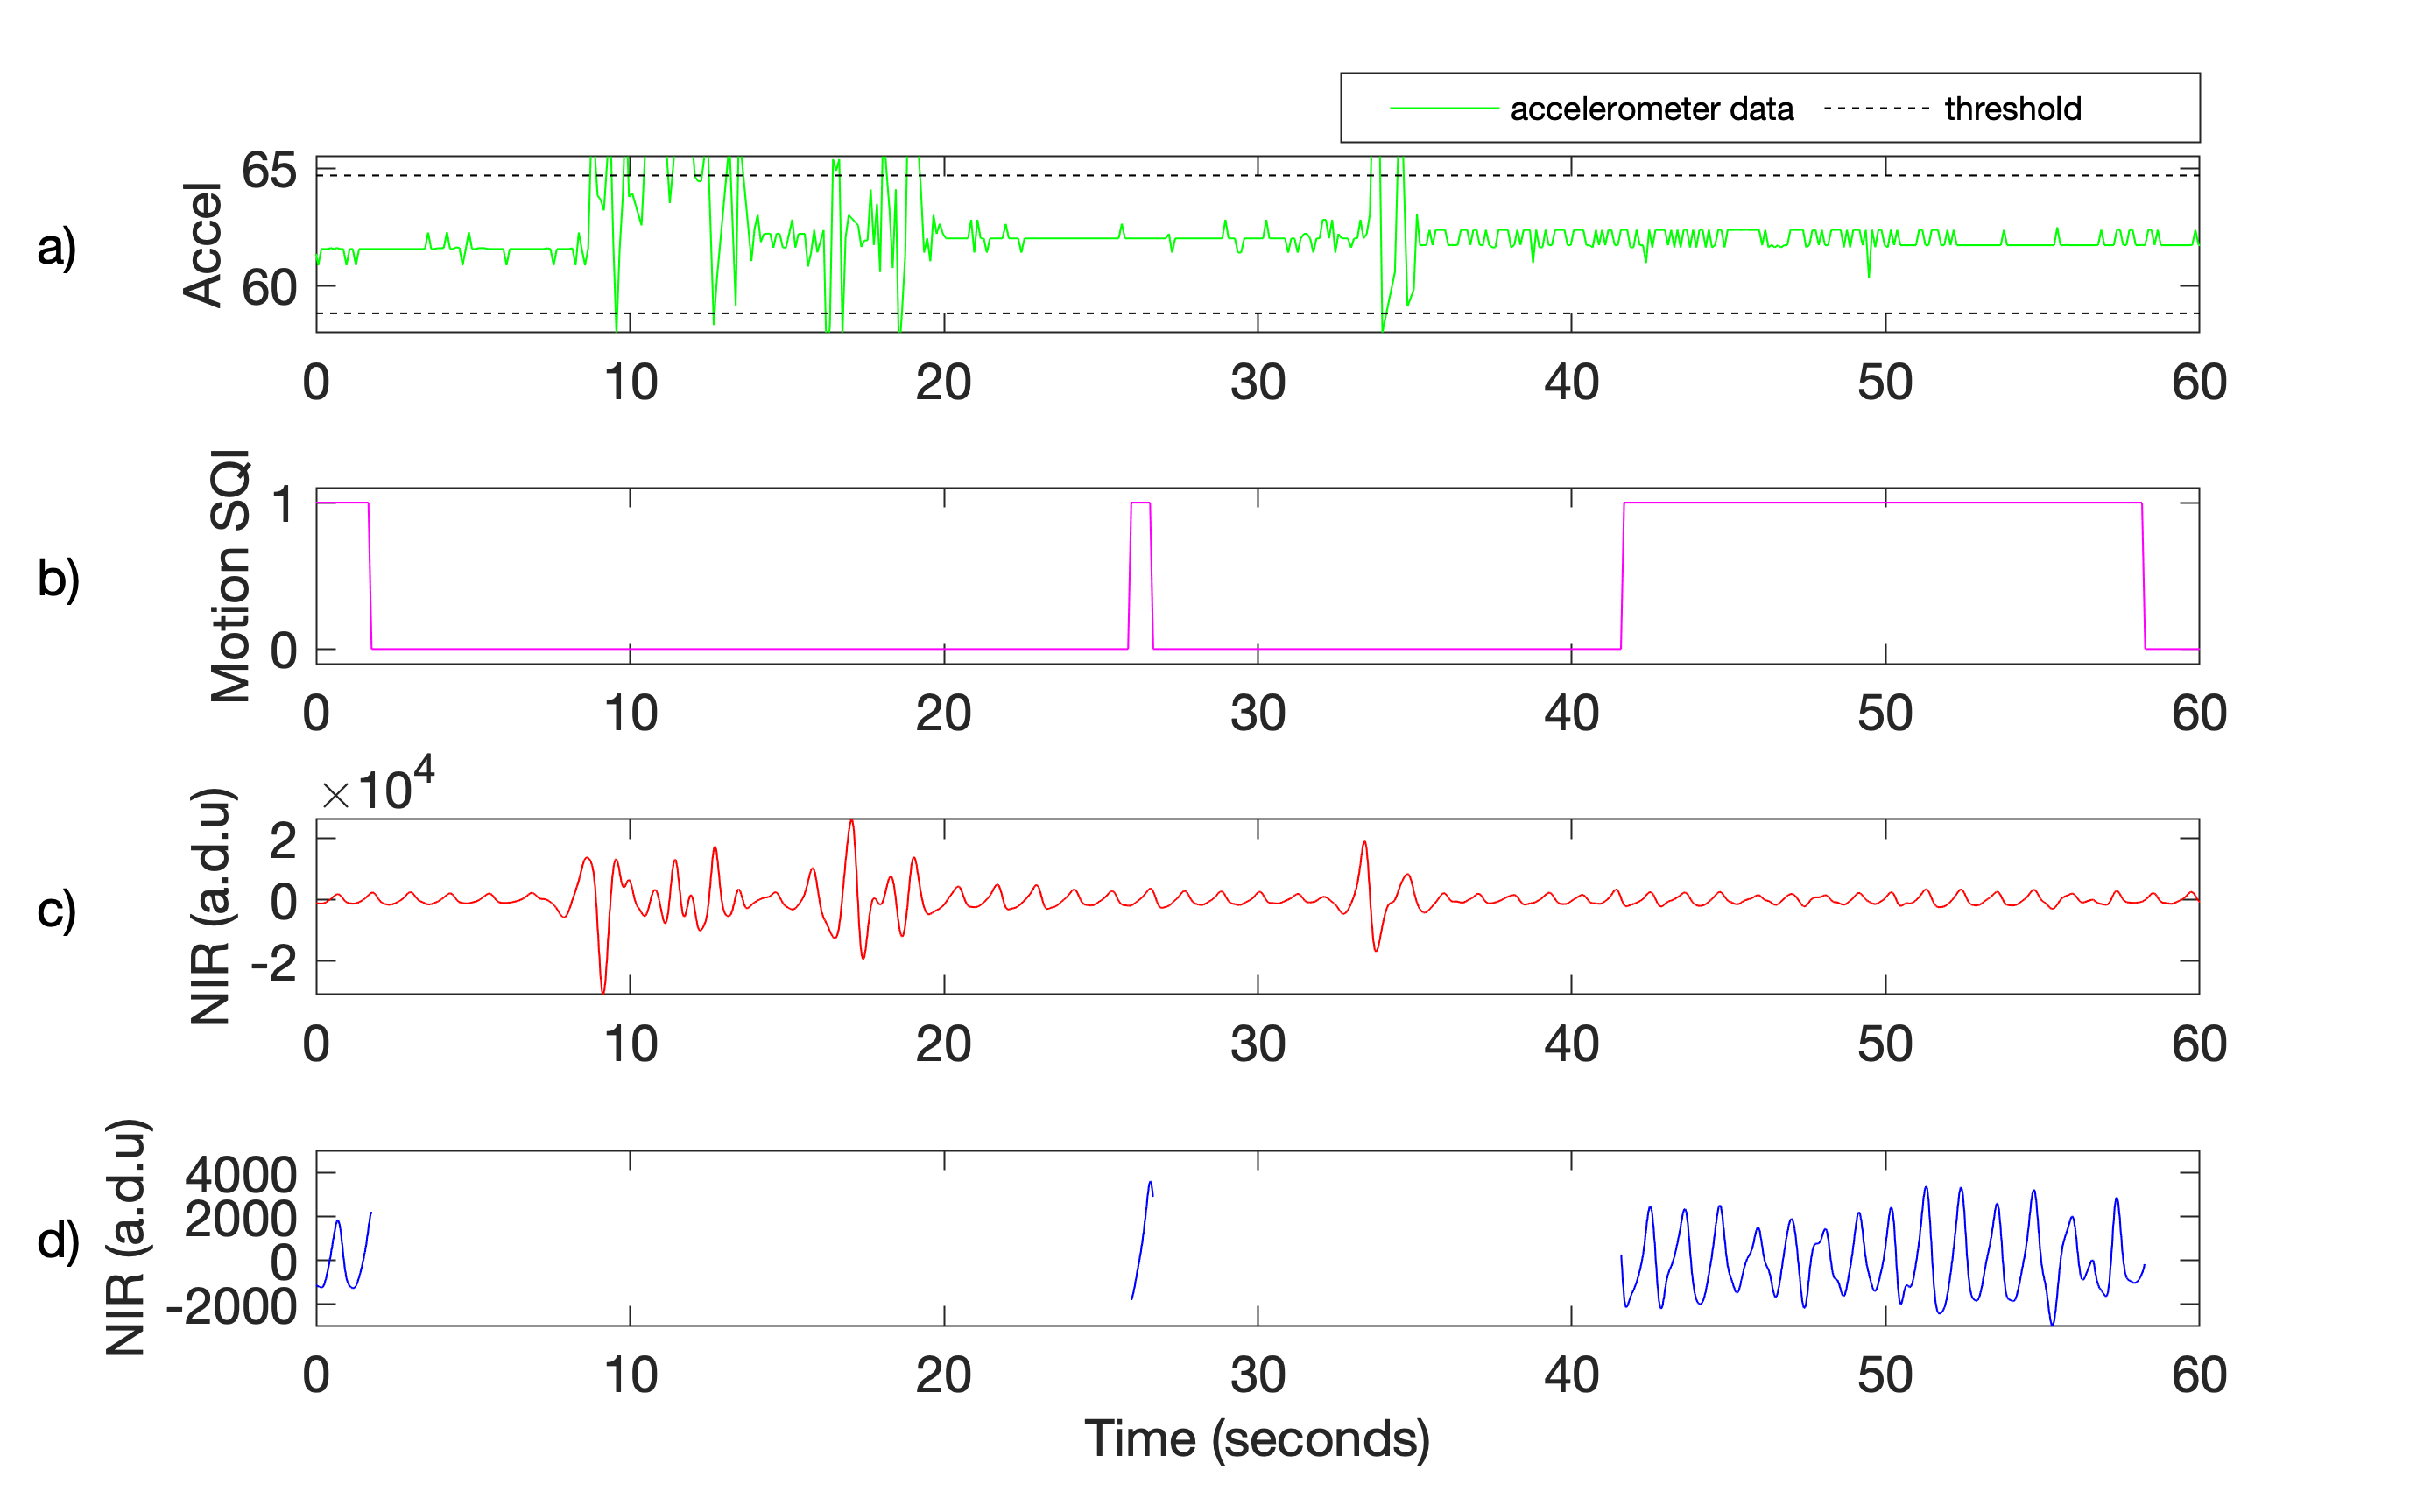
\includegraphics[width = 12 cm]{./figures/SQI.png}
    \caption[Using motion SQI to discard time periods corresponding to motion artefacts.]{Using motion SQI to discard time periods corresponding to motion artefacts. a) Accelerometer data, b) computed SQI, data is discarded at SQI = 0. c) NIR signal before motion SQI, d) NIR signal after motion SQI was applied.}
    \label{SQIACC}
\end{figure}


 
 \subsection{Heart rate computation}
 
Beat-to-beat time intervals were computed by subtracting the time value of each peak from the time value of a succeeding peak.
From the peak-to-peak intervals, HR was computed using a window length of 10 seconds sliding by 1 second. The averaged values of \gls{hr} were then calculated using the equation below:
\begin{equation}
HR = \frac{60}{median (peak\_time\_interval)}
\end{equation}
 
\subsection{Time alignment between heart rate from Philips and HR estimated from the Wavelet Health device}

The Wavelet Health and Phillips devices have separate clocks, which could not be synchronised. The time delay between devices varied session to session. To compare vital signs estimated from the Wavelet Health device to reference values from the Phillips monitor, the time delay between these devices need to be estimated and accounted for. This was accomplished by comparing the estimated \gls{hr} values from the Wavelet device with the reference \gls{hr} signal from the Phillips monitor, similar to Chaichulee \cite{chaichulee2018non}. The cross correlation between the two \gls{hr} signals was calculated for time lags from -30 s to 30 s. 

Given that $f$ and $g$ are vectors containing a time series signal, the cross-correlation measures the similarity between $f$ and a shifted version of $g$. The cross-correlation at a time lag t is defined as:

\begin{equation}
	R_{xy}(t) =\dfrac{\sum_{i-1}N(f_{i} - μ_{f}) - (g_{i-t} - μ_{g})}{(N-1) σ_{f}σ_{g}}
\end{equation}

where $μ_{f}$ and $μ_{g}$ are the means of $f$ and $g$ respectively, $σ_{f}$ and $σ_{g}$ are the variances of $f$ and $g$ respectively. The maximum of the cross-correlation indicated the time delay for which the two signals are best aligned. The time delay is defined as

\begin{equation}
  T = argmax R_{xy}(t)
\end{equation}

The time delay indicates how much $g$ is shifted, along the x-axis (time axis), with respect to $f$. Computed heart rates were then plotted and comparisons were made with the reference heart rate from the Philips monitor. 

\section{Respiratory rate estimation}
\subsection{Overview of the process}


\begin{figure}
    \centering
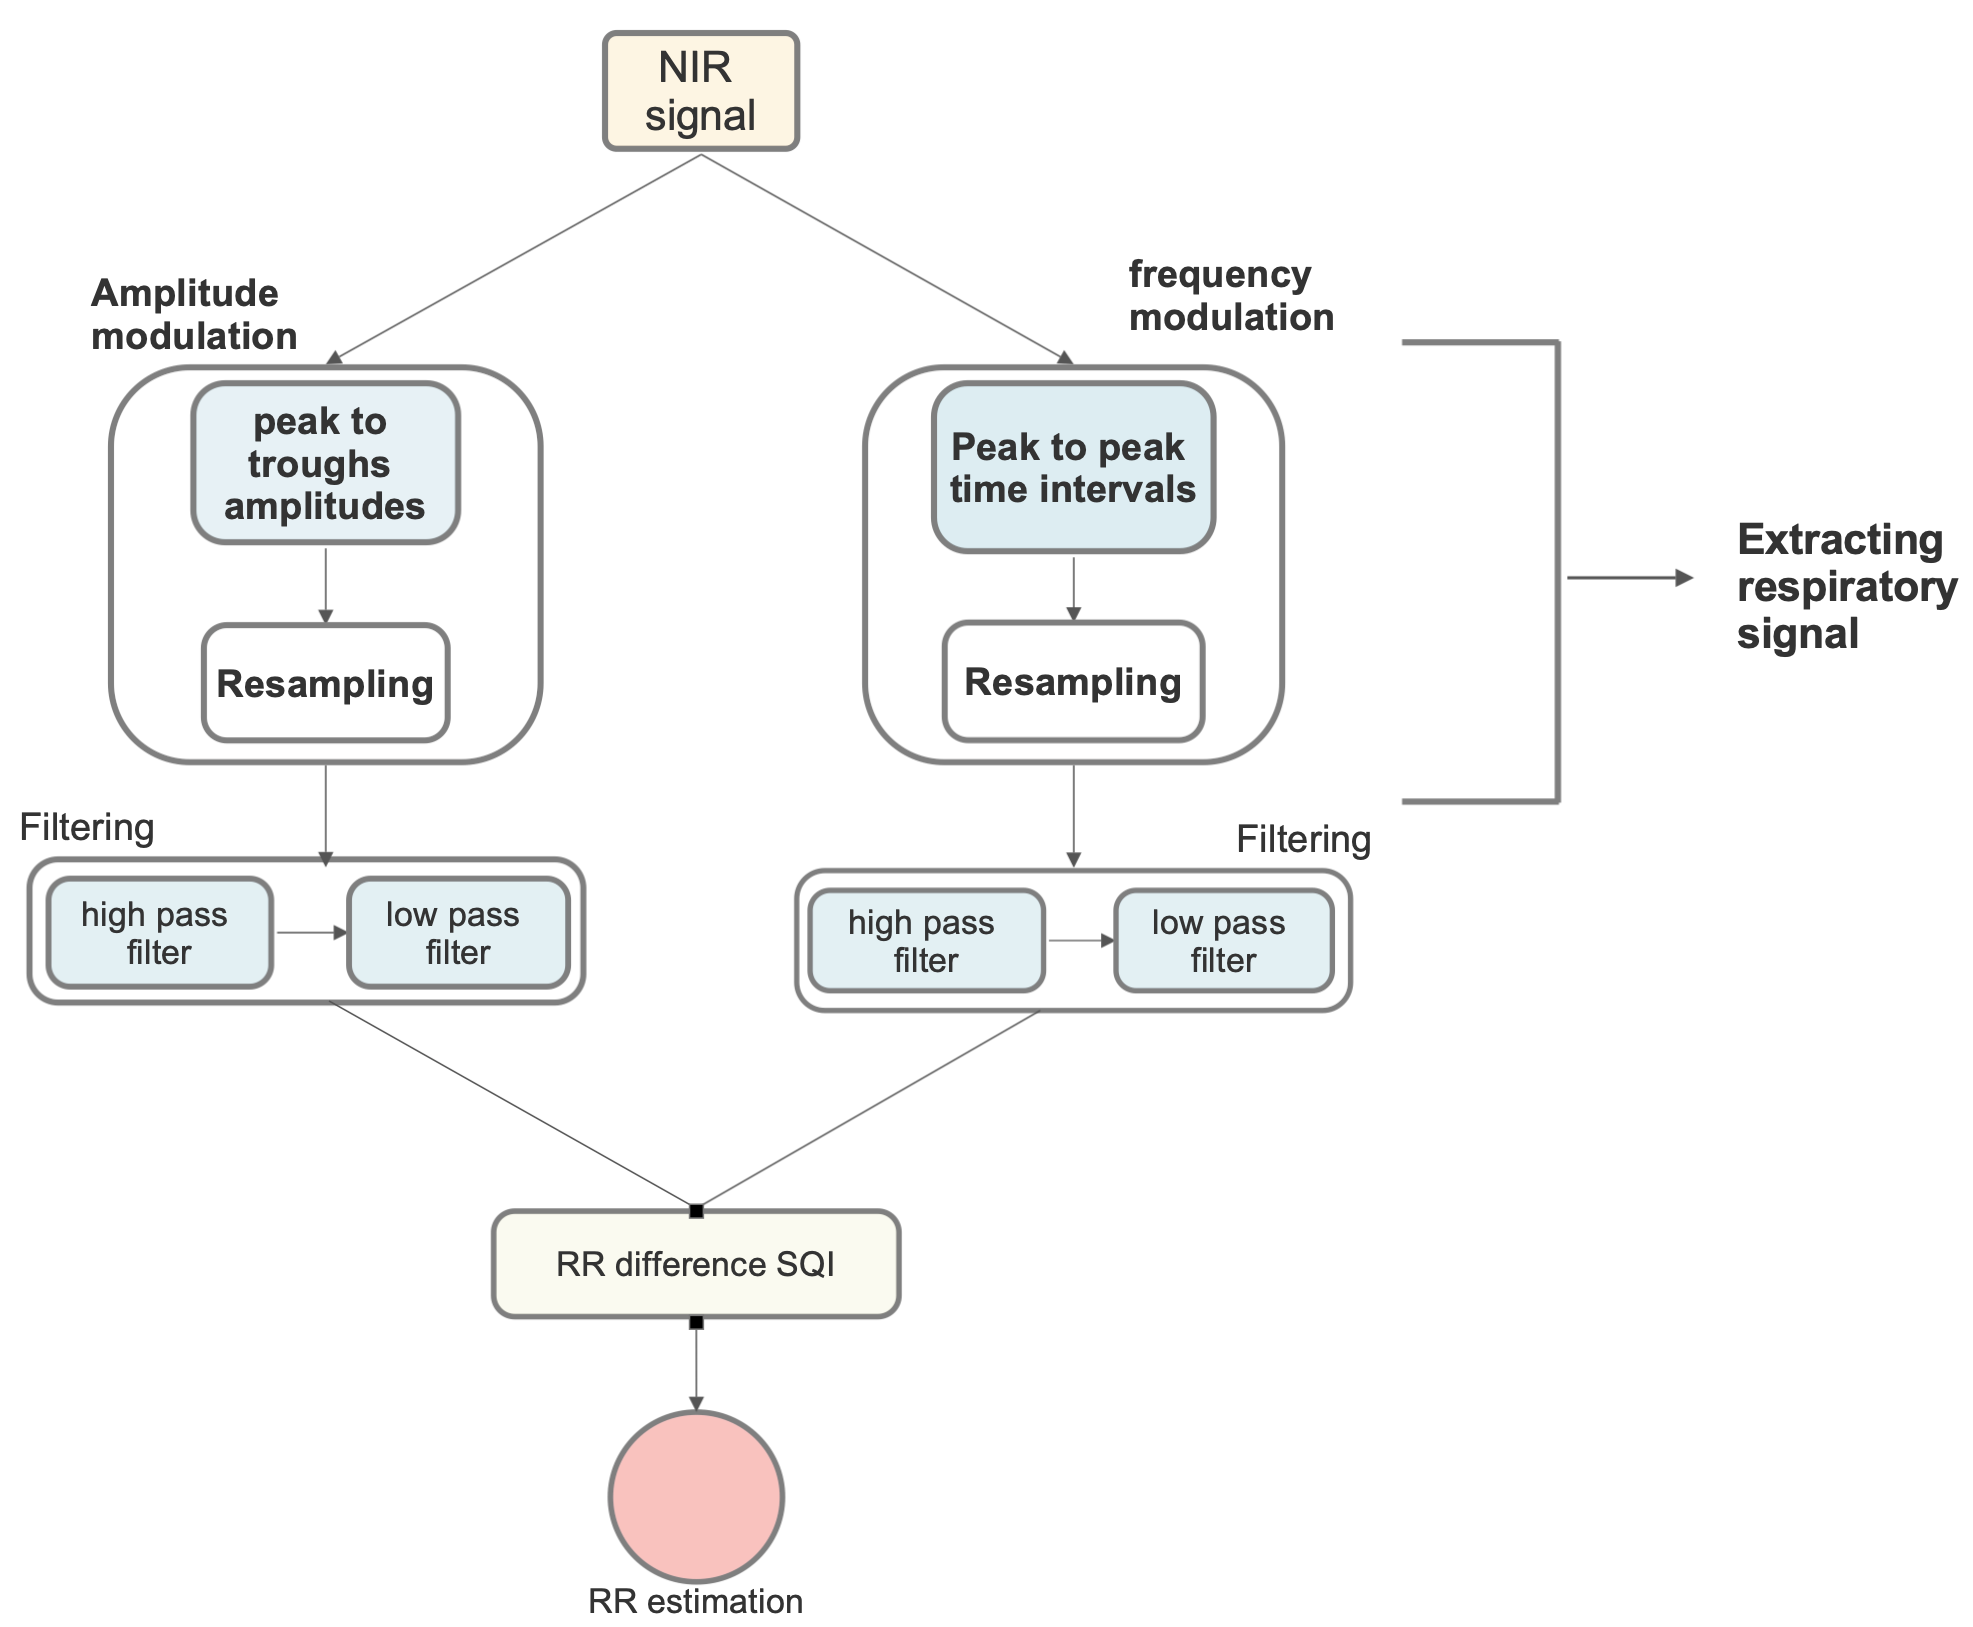
\includegraphics[width = 11 cm]{./figures/RRflowchart.png}
    \caption{Flow diagram outlining the process  of computing respiratory rate from the NIR signal recorded by the Wavelet Health wearable device.}
    \label{fig:ppg_rr_est_overview} 
\end{figure}

The estimation of respiratory rate is possible because the NIR signal recorded by the Wavelet device presents respiratory driven blood volume changes. Modulation of the NIR signal due to respiration is used to estimate RR. Two methods were used to extract a respiratory signal and compute RR from the raw NIR PPG signal. Amplitude modulation, caused by changes in intra-thoracic pressure during the respiratory cycle, resulted in respiratory oscillations in the amplitude of the signal from which RR could be estimated. The second method, frequency modulation, used the variation in the instantaneous heart rate during the respiratory cycle, also known as respiratory-sinus arrhythmia. The extracted respiratory signals were filtered using two zero-phase Infinite Impulse Response (IIR) filters. The mean of the two filtered respiratory signals was taken as the final estimate of RR.

\subsection{Extracting respiratory signal}

\subsubsection{Amplitude modulation}

Amplitude modulation is defined as the difference in peak amplitudes of consecutive peaks and troughs, effectively resulting in a time-series of the amplitude of each PPG pulse.
It is caused directly by changes in intra-thoracic pressure during the respiratory cycle. These changes result in respiratory oscillations in the amplitude of the signal, from which RR can be estimated. 

For this method, the peaks and troughs of the NIR signal were computed using the algorithm described in section~\ref{fig:ppg_rr_est_overview}, as shown in figure~\ref{amplimod}a. The amplitude of each beat was computed by subtracting the trough values from each respective peak. Outliers, defined as values more than three standard deviations from the mean, were removed from the peak-trough amplitudes to discard noisy periods. The signal was then re-sampled at 25 Hz (using a cubic spline), and de-trended as shown ~\ref{amplimod}b and ~\ref{amplimod}c. 


\begin{figure}
    \centering
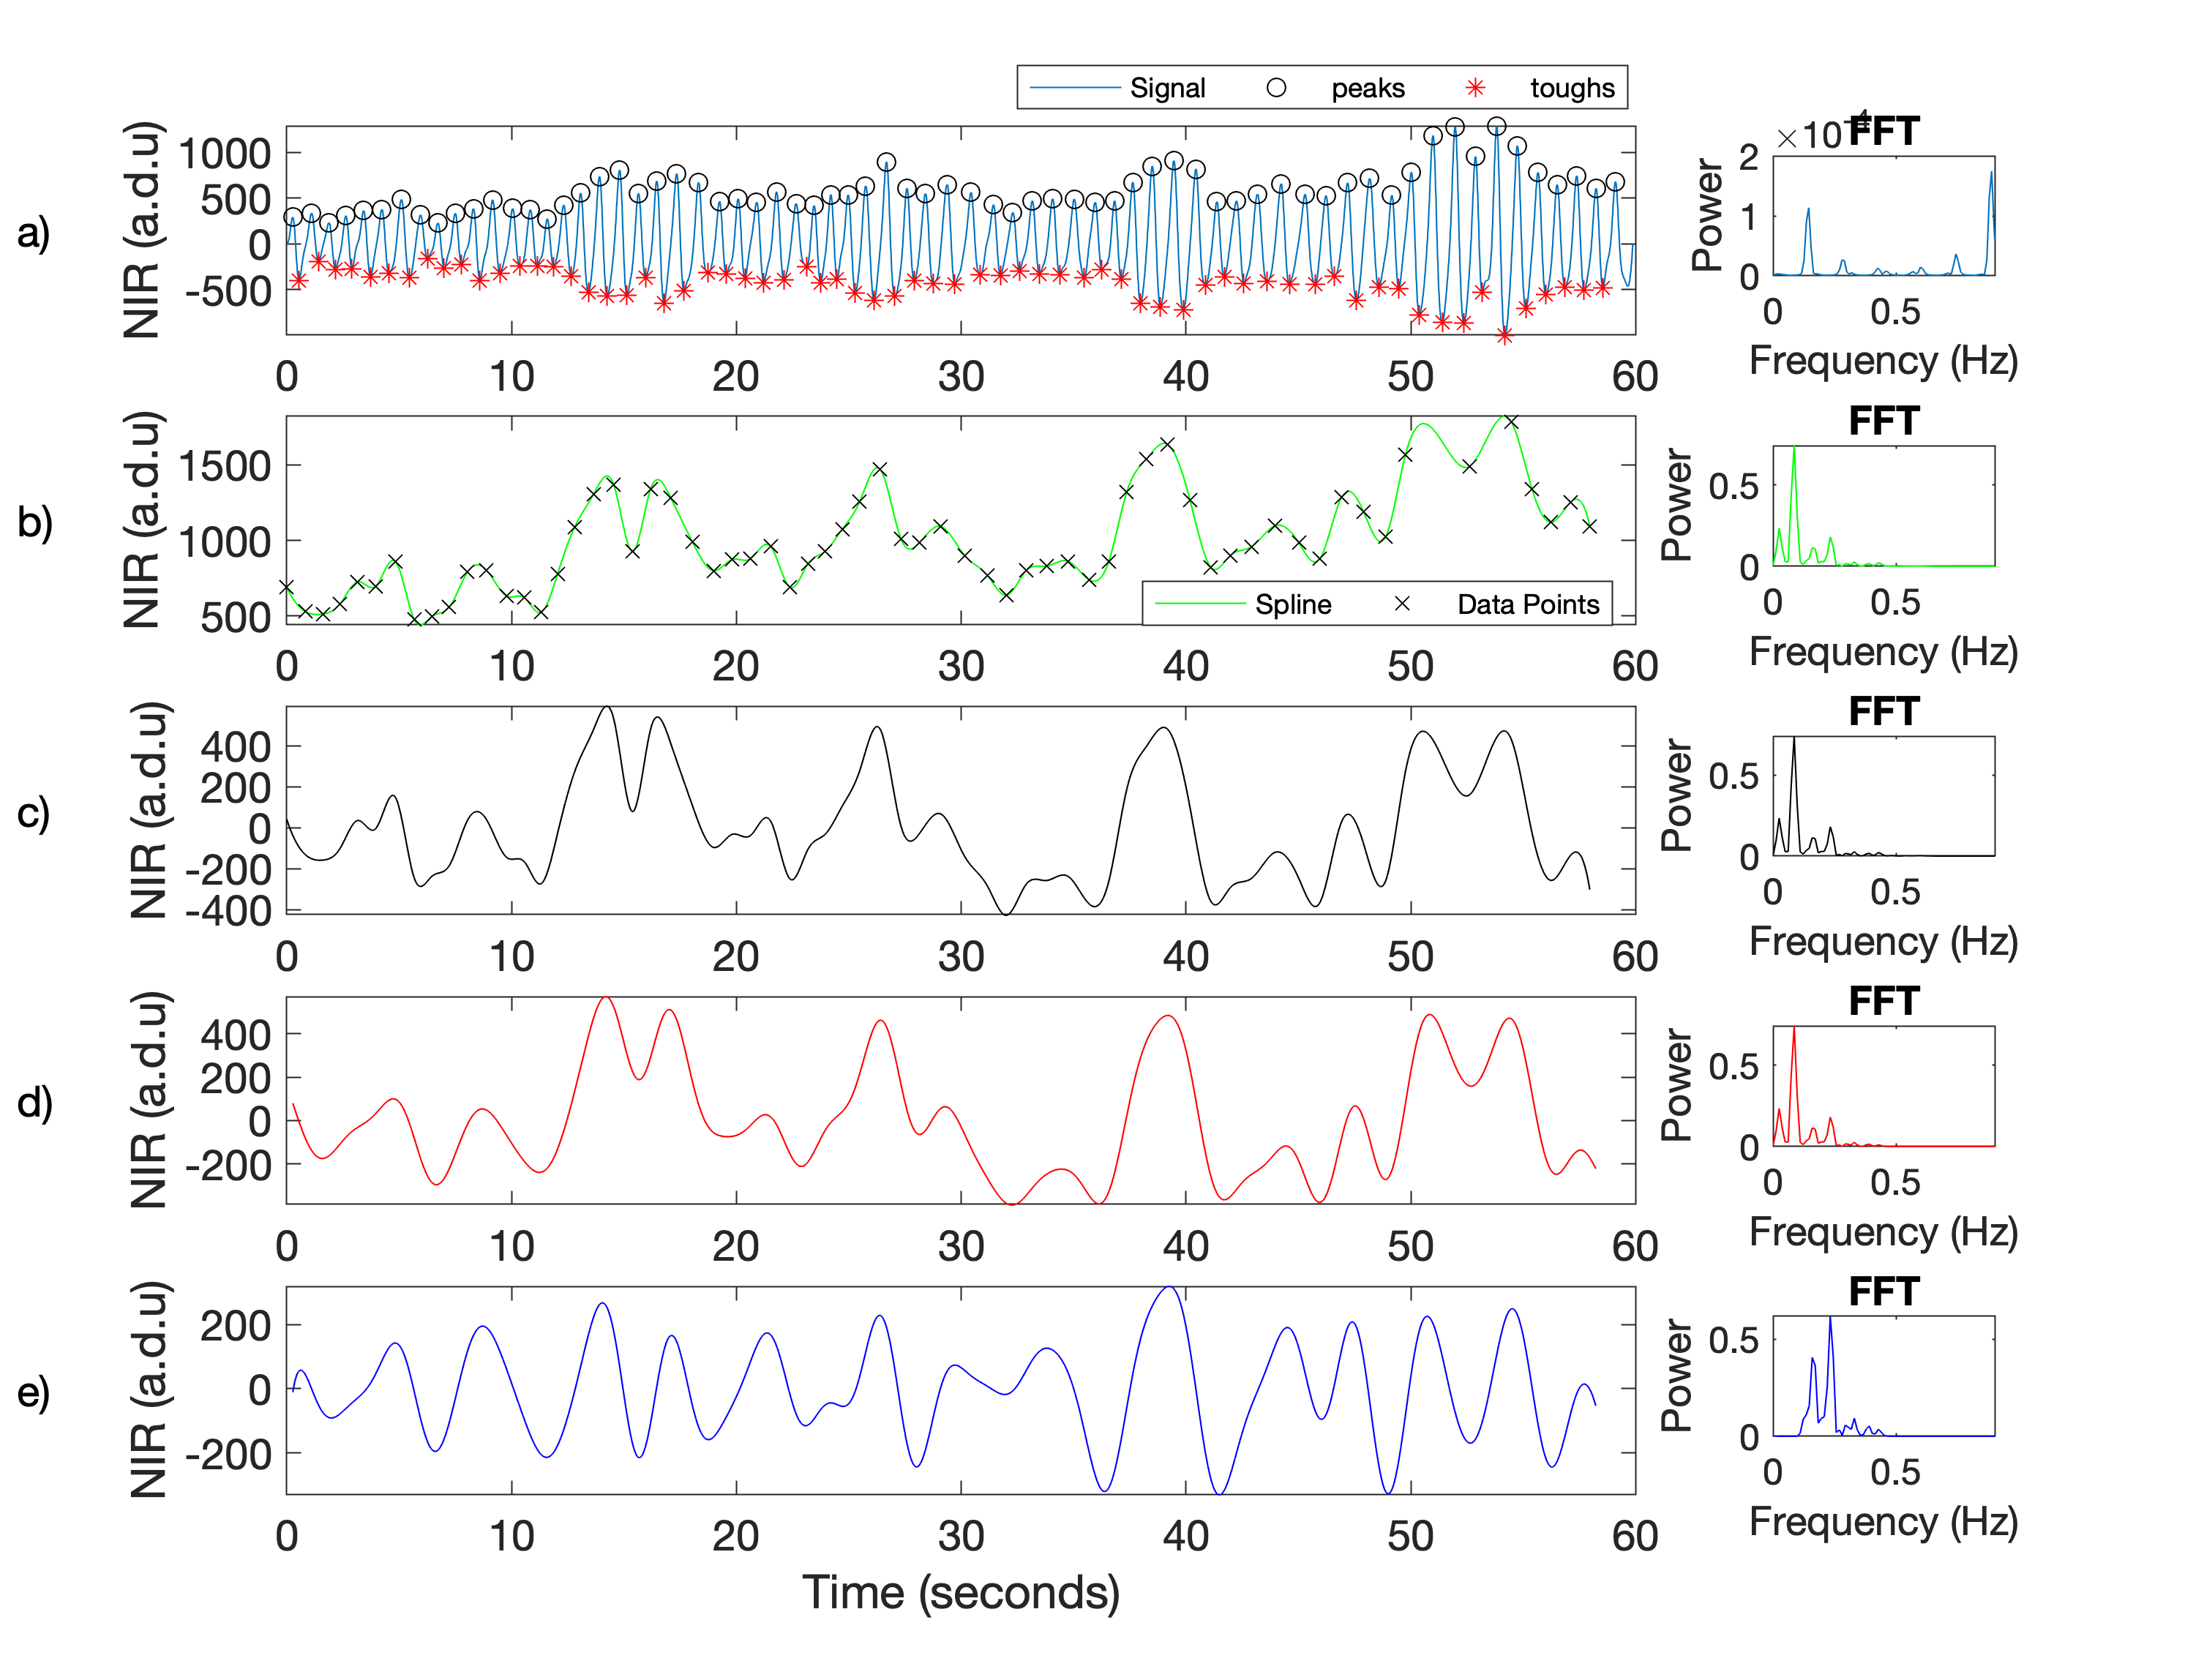
\includegraphics[width = 12 cm]{nicu_Amplimod.png}
    \caption[60-second example of the amplitude modulation method being used to estimate RR from the NIR signal.]{60-second example of the amplitude modulation method being used to estimate RR from the NIR signal. a) Peak-to-trough detection; b) signal amplitude; c) de-trended; d) low-pass filtered signal; e) high-pass filtered signal. The FFT panels show a peak at 0.23Hz, corresponding to a RR of approximately 13.8 breaths/minute. The reference RR recorded by the Philips monitor was 15 breaths/minute.}
    \label{amplimod} 
\end{figure}


Two Butterworth IIR filters shown in figure~\ref{mag_RRresampled}, were designed to remove low and high frequency noise from the signal. An $8_{th}$ order low-pass filter was designed with a cut-off frequency of 0.60 Hz (36 breaths/min) and a passband frequency of 0.40 Hz (24 breaths/min). A high-pass filter of order 17 with a passband frequency of 0.12 Hz (7.2 breaths/min) and a cut-off frequency of 0.10 Hz (6 breaths/min) was then applied to the signal. Both filters were designed with a passband ripple of 1 dB and stop band attenuation of 20 dB. Figure ~\ref{amplimod} shows an example plot of the NIR signal before and after de-trending and filtering. The designed filters were used to remove low and high frequency noise from the signal as shown in figure ~\ref{amplimod}d and ~\ref{amplimod}e. 


\begin{figure}
\centering
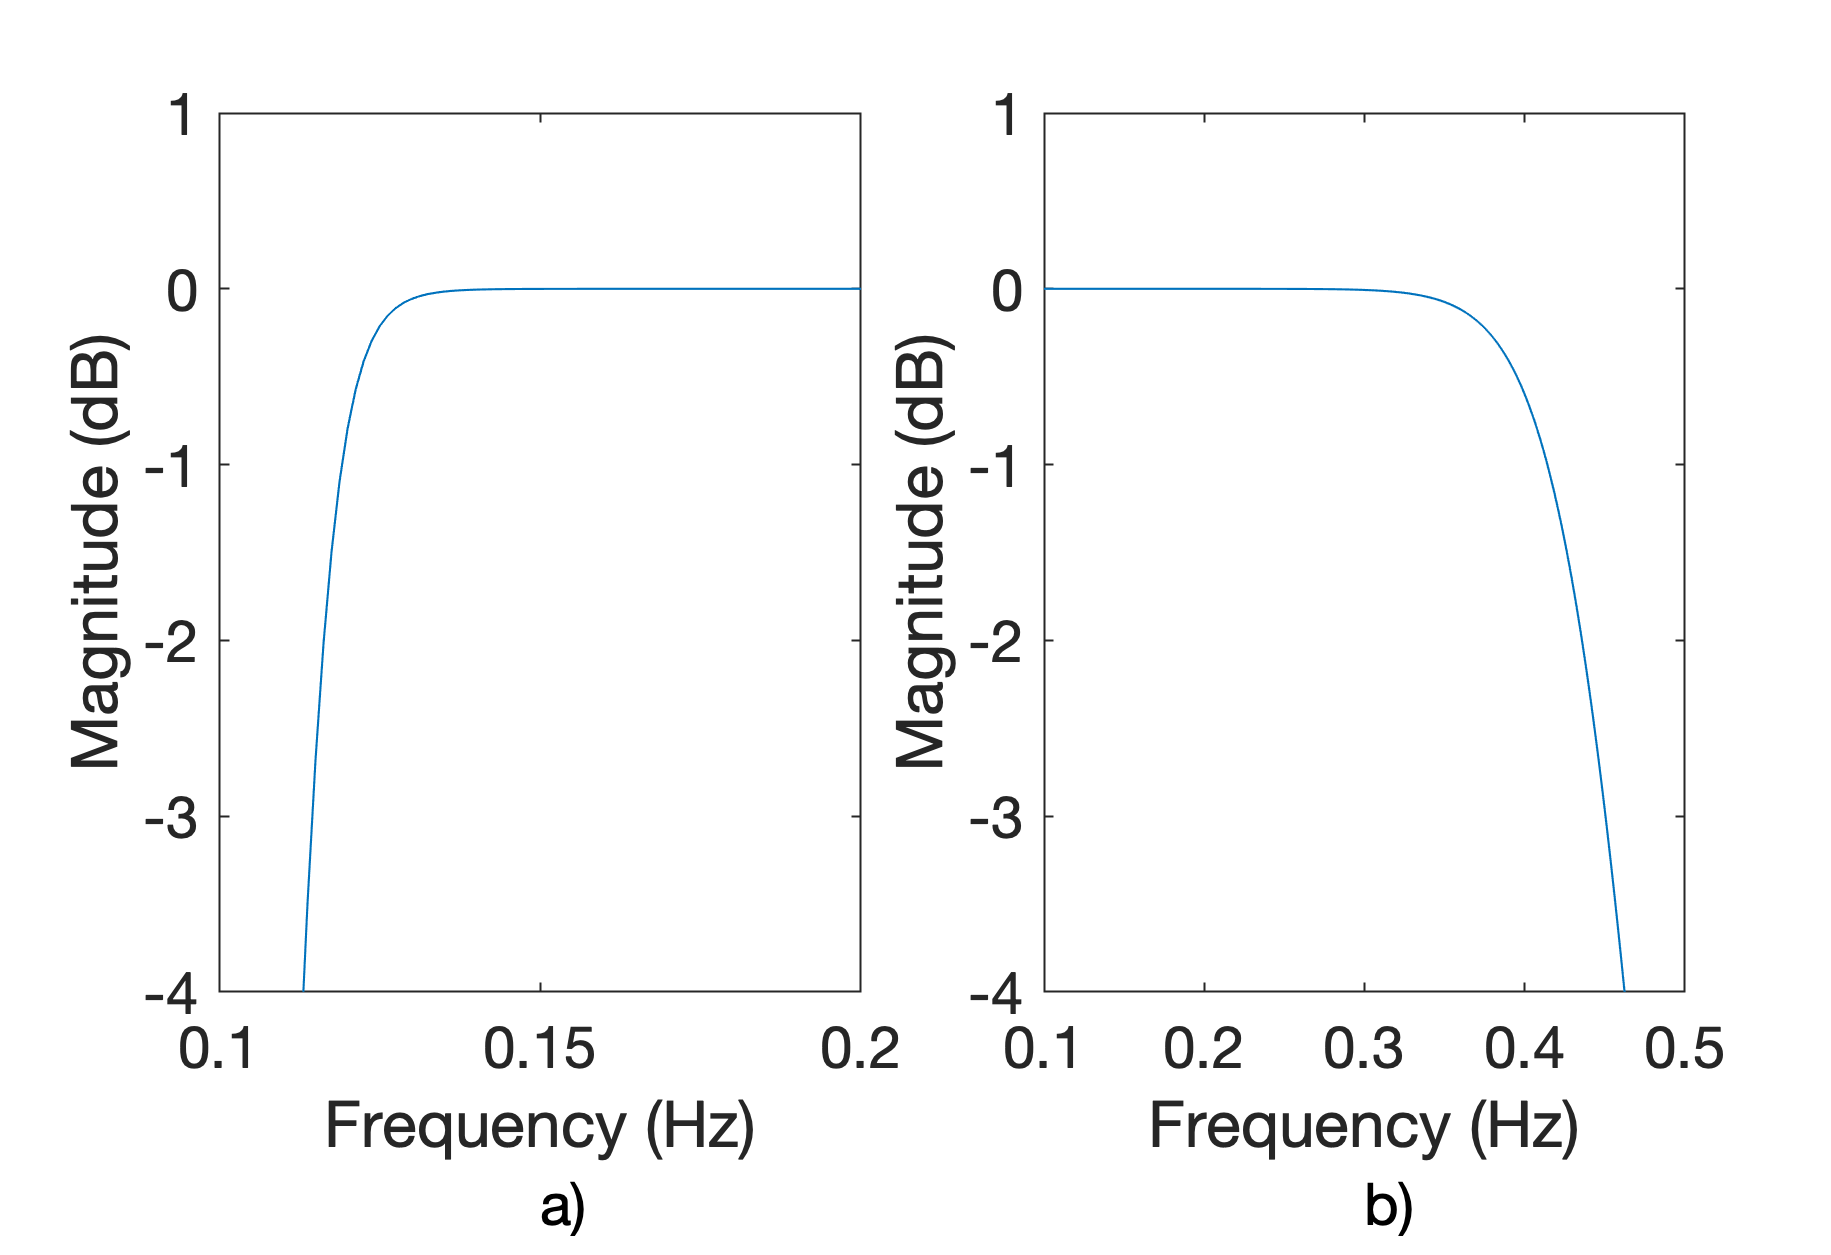
\includegraphics[width = 10 cm]{./figures/mag_resampledrr.png}
    \caption[Filter magnitude responses.]{Filter magnitude responses for a) high-pass filter b) low-pass filter.}
        \label{mag_RRresampled}
\end{figure}


\subsubsection{Frequency modulation} 

Frequency modulation, also known as respiratory sinus arrhythmia, is a variation in heart rate that occurs throughout the respiratory cycle. It is well documented that heart rate increases during inspiration and decreases during expiration. While the precise mechanisms of frequency modulation remain disputed, it is a result of autonomic nervous system activity fluctuation during respiration.

To compute RR using this method, peak to peak time intervals were computed by subtracting the peak time point from a succeeding peak. The peak-to-peak time intervals for each breath pulse from the NIR signal were extracted to construct a respiratory signal. The signal was re-sampled at 25Hz (using a cubic spline). Subsequently, the detrended signal was filtered using similar filters designed for the amplitude modulation method. The peak-to-peak time intervals were then used to compute RR. An example from this process is shown in figure~\ref{Freqmod}. The FFT panels show a peak at 0.24Hz, corresponding to a RR of 14.4 breaths/minute. The reference RR recorded by the Philips monitor was 15 breaths/minute.


\begin{figure}
    \centering
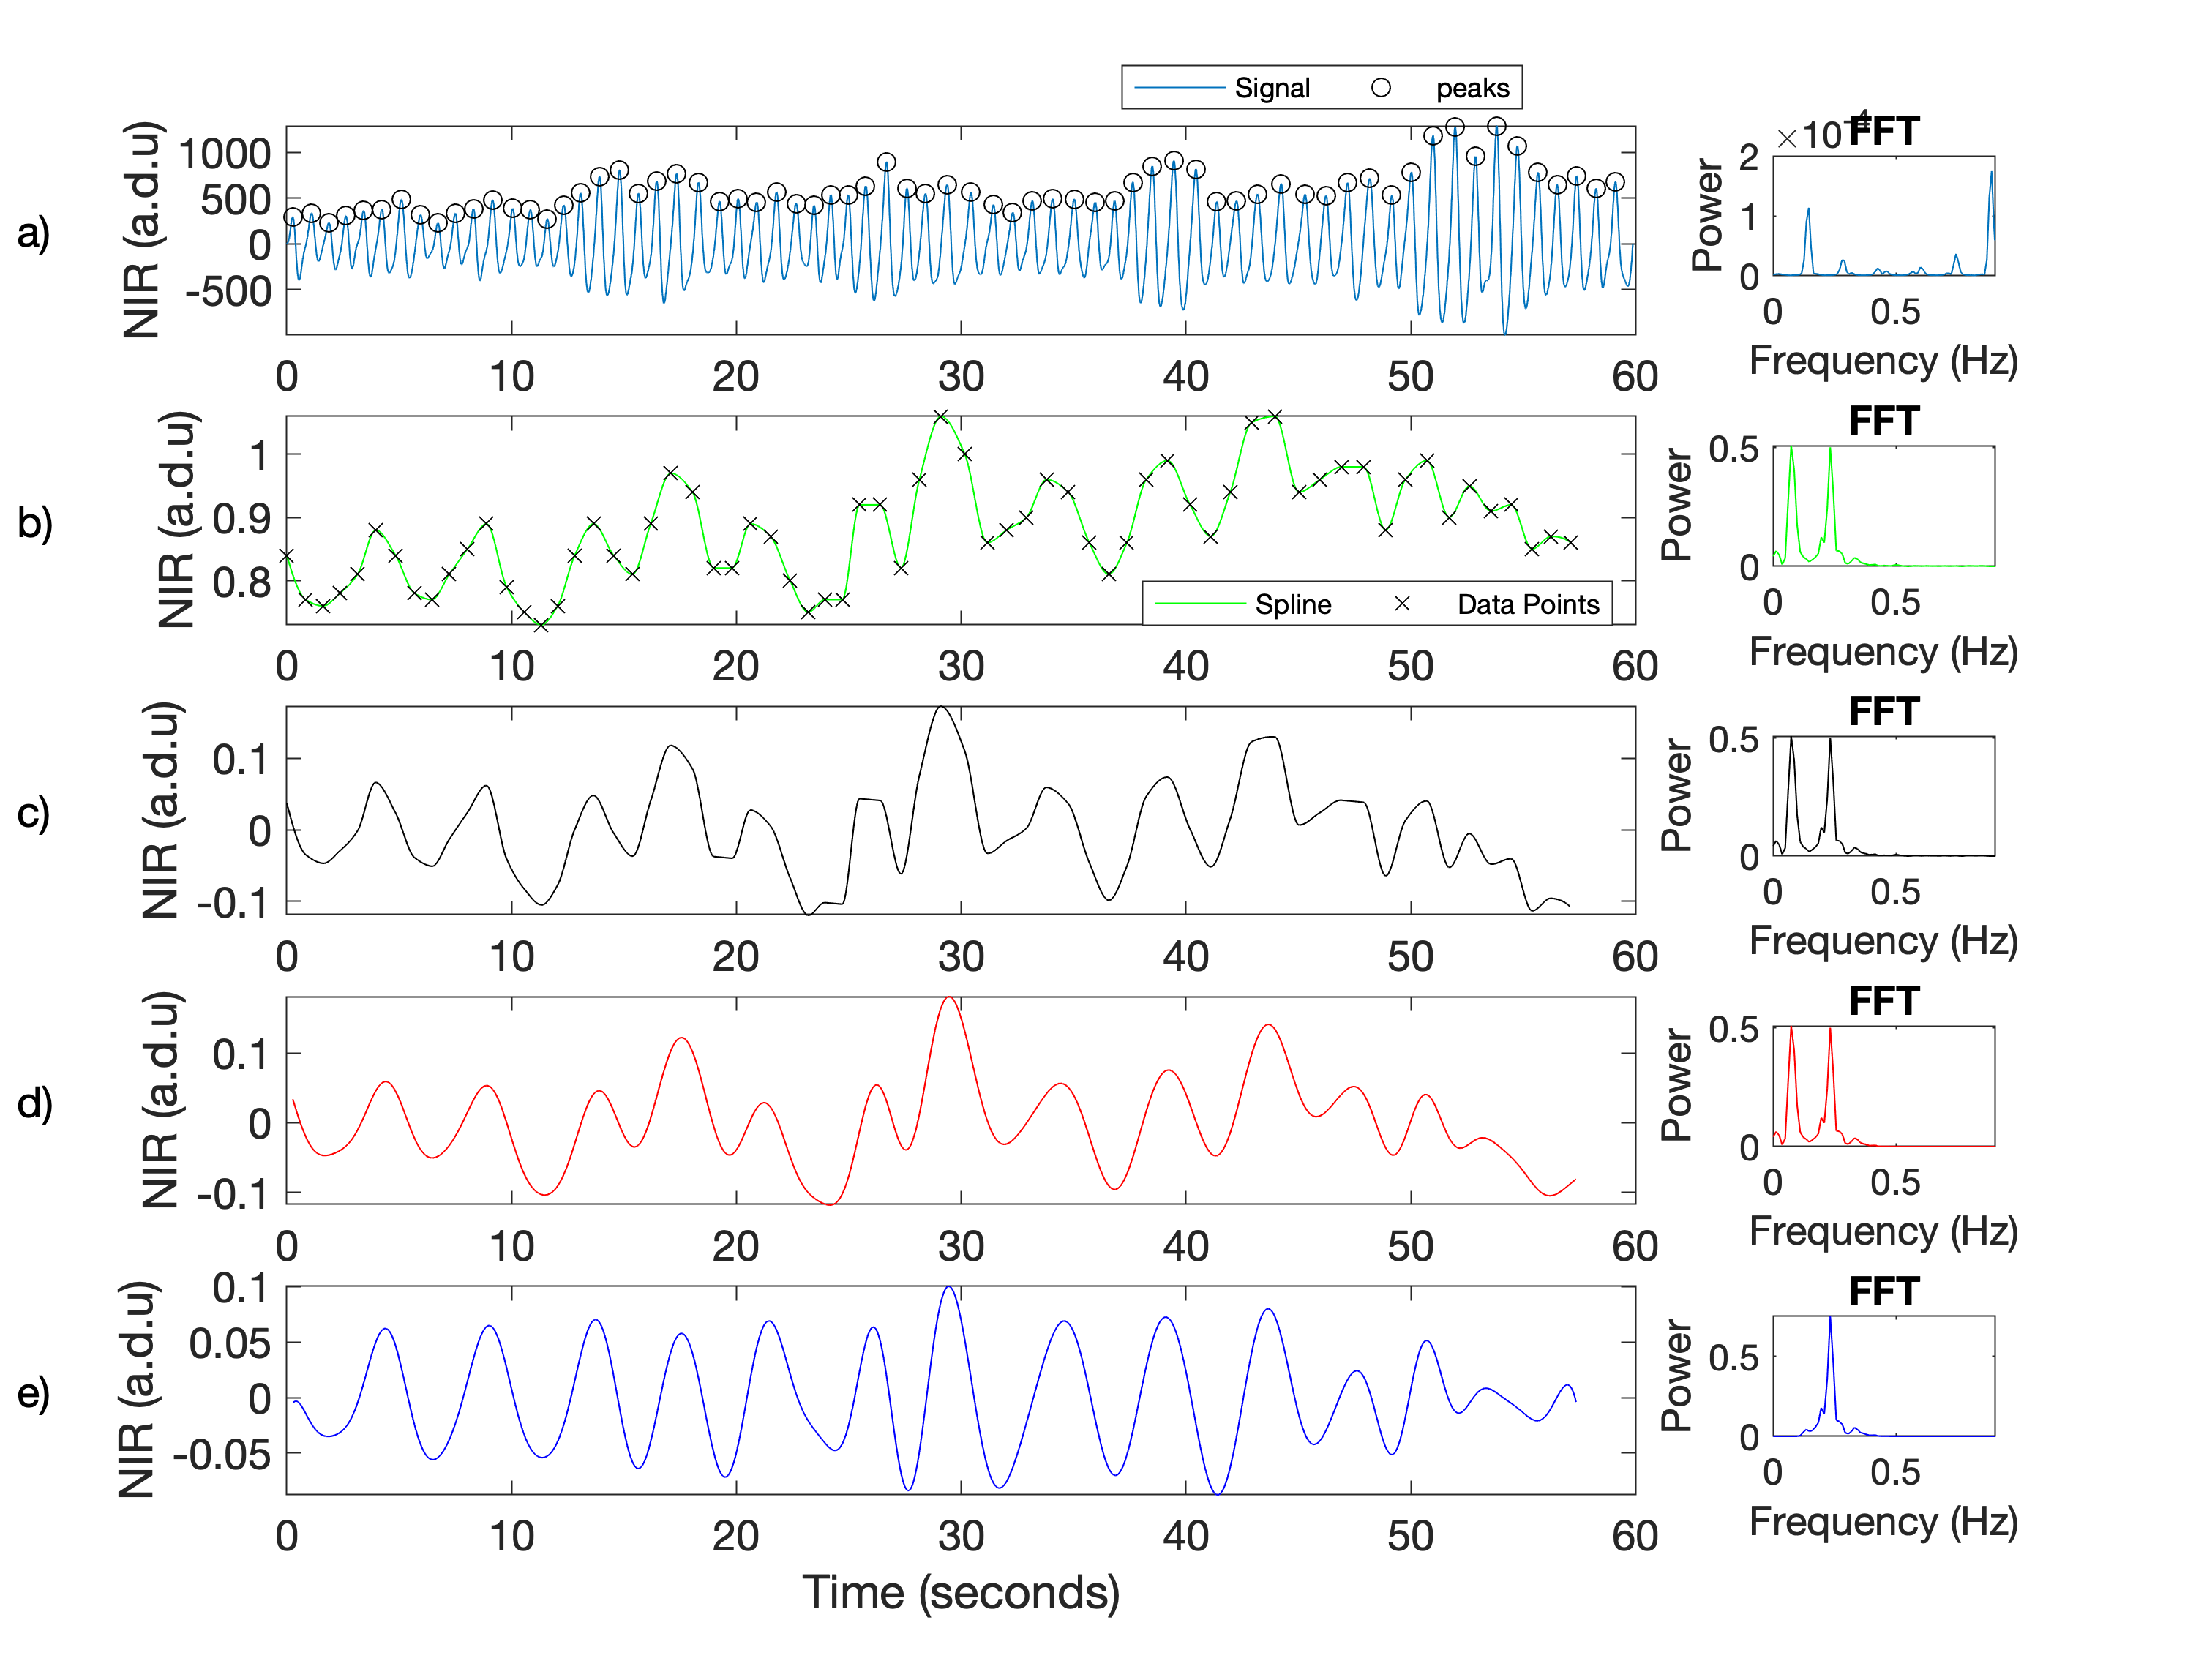
\includegraphics{nicu_Freqmod.png}
    \caption [60-second example of the frequency modulation method used to estimate RR from the NIR signal.]{60-second example of the frequency modulation method used to estimate RR from the NIR signal. a) Peak to peak time intervals; b) peak to peak time intervals; c) de-trended; d) low-pass filtered signal; e) high-pass filtered signal. The FFT panels show a peak at 0.24Hz, corresponding to a RR of 14.4 breaths/minute. The reference RR recorded by the Philips monitor was 15 breaths/minute.}
    \label{Freqmod} 
\end{figure}


\subsection{RR estimation}

To compute RR, similar algorithms described in section ~\ref{peak_eqn} were used to perform peak to peak analysis on the respiratory signals extracted from the NIR waveform using both of the proposed methods. This analysis was done using MinPeakDistance of 1.2 s (50 breaths/min) and MinPeakProminence of 0.02. \gls{rr} was computed as the average peak-to-peak time interval over a window of 30 seconds sliding by 5 seconds. The agreement between the estimated \gls{rr} from the two methods (amplitude and frequency modulation) was used to compute an SQI. This SQI was set to 1, corresponding to periods of good quality estimates, if the two estimates were within 5 breaths/min; conversely, it was set to 0 otherwise, corresponding to time periods of poor-quality estimates. The mean of the two respiratory rates was taken as the final estimate of \gls{rr} for periods of good-quality signal.

\section{Oxygen saturation}
\subsection{Overview of the process}

The Wavelet Health device, although it provided estimates of HR, also recorded the red and NIR signals. These signals were split into windows, and then detrended and filtered to remove noise. Subsequently, a motion SQI was applied using accelerometer data to remove data where the red and NIR signals were corrupted by motion. After this, the peaks and troughs in the red and NIR signals were detected, and the signal amplitude computed. The ratio between the red and NIR signal amplitudes were then compared to the reference \gls{$SpO_{2}$} estimates from the Philips monitor. This process is shown in figure~\ref{spo2flow}. 


\begin{figure}
  \centering
    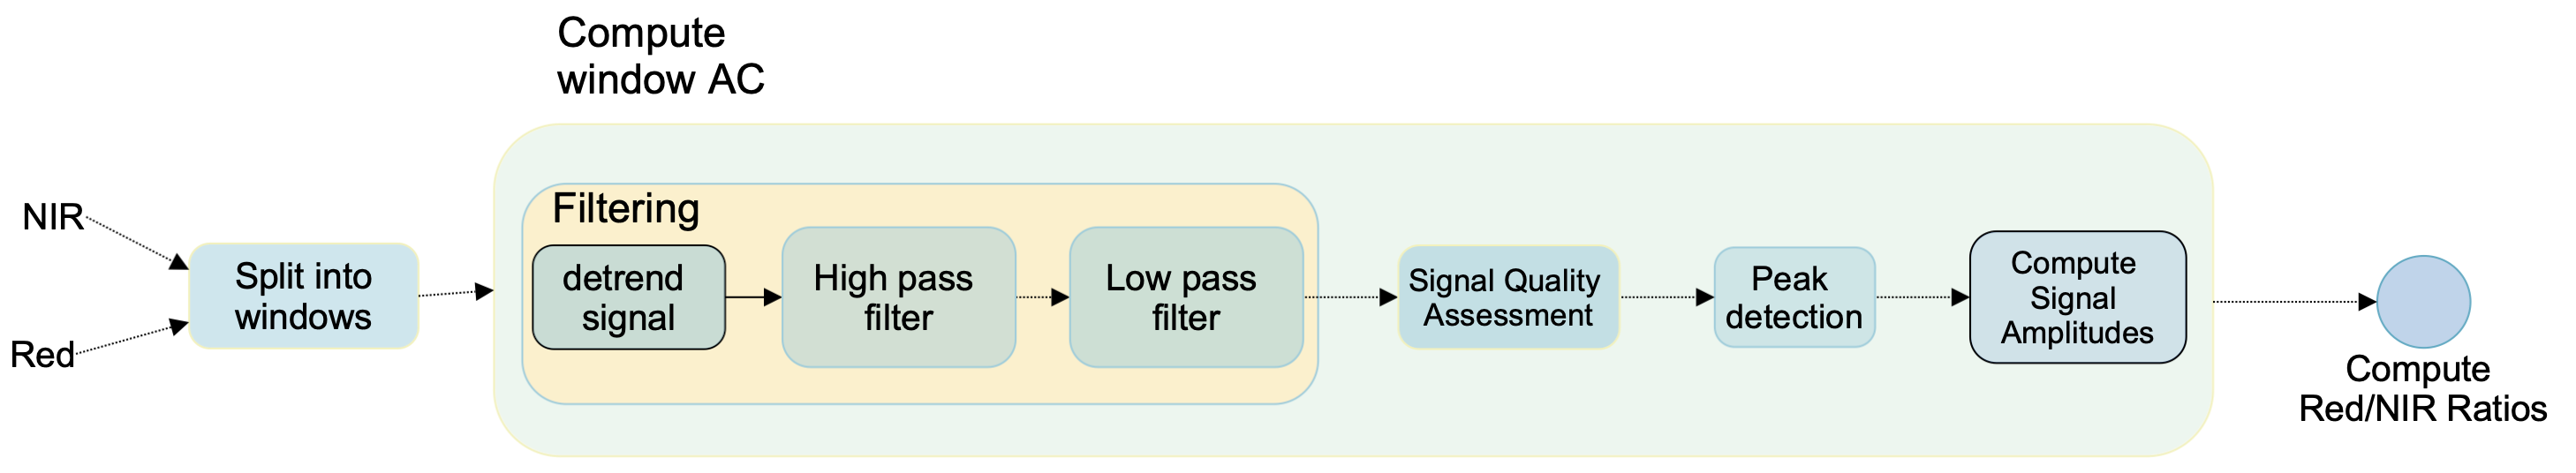
\includegraphics{nicu_SpO2flowchart.png}
    \caption{Flow diagram outlining the process of computing the relationship between the ratio of ratios of the red and NIR signals recorded by the Wavelet Health device and the reference \gls{$SpO_{2}$} from the Philips monitor.}
        \label{spo2flow}
\end{figure}


\subsection{Filtering}

The NIR and Red signals were de-trended and subsequently filtered using two zero-phase FIR filters with a passband ripple of 1dB and stop band attenuation of 20dB to remove low and high frequency noises from the signal respectively. The high-pass filter was designed with a passband frequency of  0.7Hz (42 beats/min) and a stop-band frequency of 0.3Hz (18 beats/min)). The low-pass filter was designed with a passband frequency of 2Hz (120 beats/min)) and a stop-band frequency of 4Hz (240 beats/min)). Thresholds were selected based on the population distribution of data shown in figure~\ref{vs hist}. The magnitude response of the resulting filters is shown in figure~\ref{mag_Spo2}. 

\begin{figure}
\centering
\includegraphics[width = 10 cm]{./figures/mag_responsehr.png}
    \caption[Magnitude responses.]{Magnitude responses for the a) High-pass filter and b) low-pass filter designed.}
        \label{mag_Spo2}
\end{figure}

Motion SQI and peak detection algorithms similar to those used in section~\ref{HR est_wav} were then applied to the filtered data.

\subsection{Signal amplitude}

The detected peaks and troughs used for \gls{hr} were used to compute the amplitude of the red and NIR PPG signals. Amplitudes were determined by consistently subtracting the value of a trough from the value of a preceeding peak.

\subsection{Computing Red/NIR Ratios}

Median values of the red and NlR PPG amplitudes were computed for non-overlapping windows of length 15 second and with 15 second step size. The ratio between the red and NIR PPG amplitudes was then applied.
For comparison, the median of 15 second non-overlapping windows were also computed from the reference \gls{$SpO_{2}$} values recorded by the Philips monitor data. The computed Red/NIR ratios were then compared to the median \gls{$SpO_{2}$} values to assess the correlation. 

 \section{Results}
 
 \subsection{Error metrics}
 
The comparison between the reference values from the Philips monitor and the estimated vital signs from the Red and NIR signals for all recordings in the study were performed using Bland-Altman analysis, the mean absolute error (MAE), the mean absolute deviation (MAD) and Pearson's correlation coefficients. The Bland-Altman plot was designed to assess the agreement between two clinical \linebreak measurements. It was constructed by plotting the mean of the estimates  from the devices against their differences. 

Given two time series x and y of length N , the MAE was defined as:

\begin{equation}
MAE = \frac{1}{N}\sum_{i=1}^{N} |y-x|
\end{equation}

Given z is the difference between the two time series x and y, and μ is the mean of z, the MAD was defined as:

\begin{equation}
MAD = \frac{1}{N}\sum_{i=1}^{N} |z-u|
\end{equation}

The Root Mean square error (RMSE) was calculated using the equation

\begin{equation}
RMSE = \sqrt{\frac{1}{N}\sum_{i=1}^{N} (y-x)^{2}}
\end{equation}

The Pearson's correlation coefficient measures the linear correlation between two time series using the following equation:
\begin{equation}
R = \frac{\mathbf{cov}(x, y)}{\sigma_{x} \times \sigma_{y}}
\end{equation}

where $\mathbf{cov}(x, y)$ is the covariance, $\sigma_{x}$ and $\sigma_{y}$ are the standard deviation of x and y time series respectively. 
  
 \subsection{Heart rate}
 
 Figure~\ref{HRseries} compares the reference HR from the Philips monitor with the estimated HR from the Wavelet Health device. Table \ref{metrics} shows MAE, MAD, RMSE values and the correlation values computed across the 10 subjects selected for analysis. 


\begin{figure}
\centering
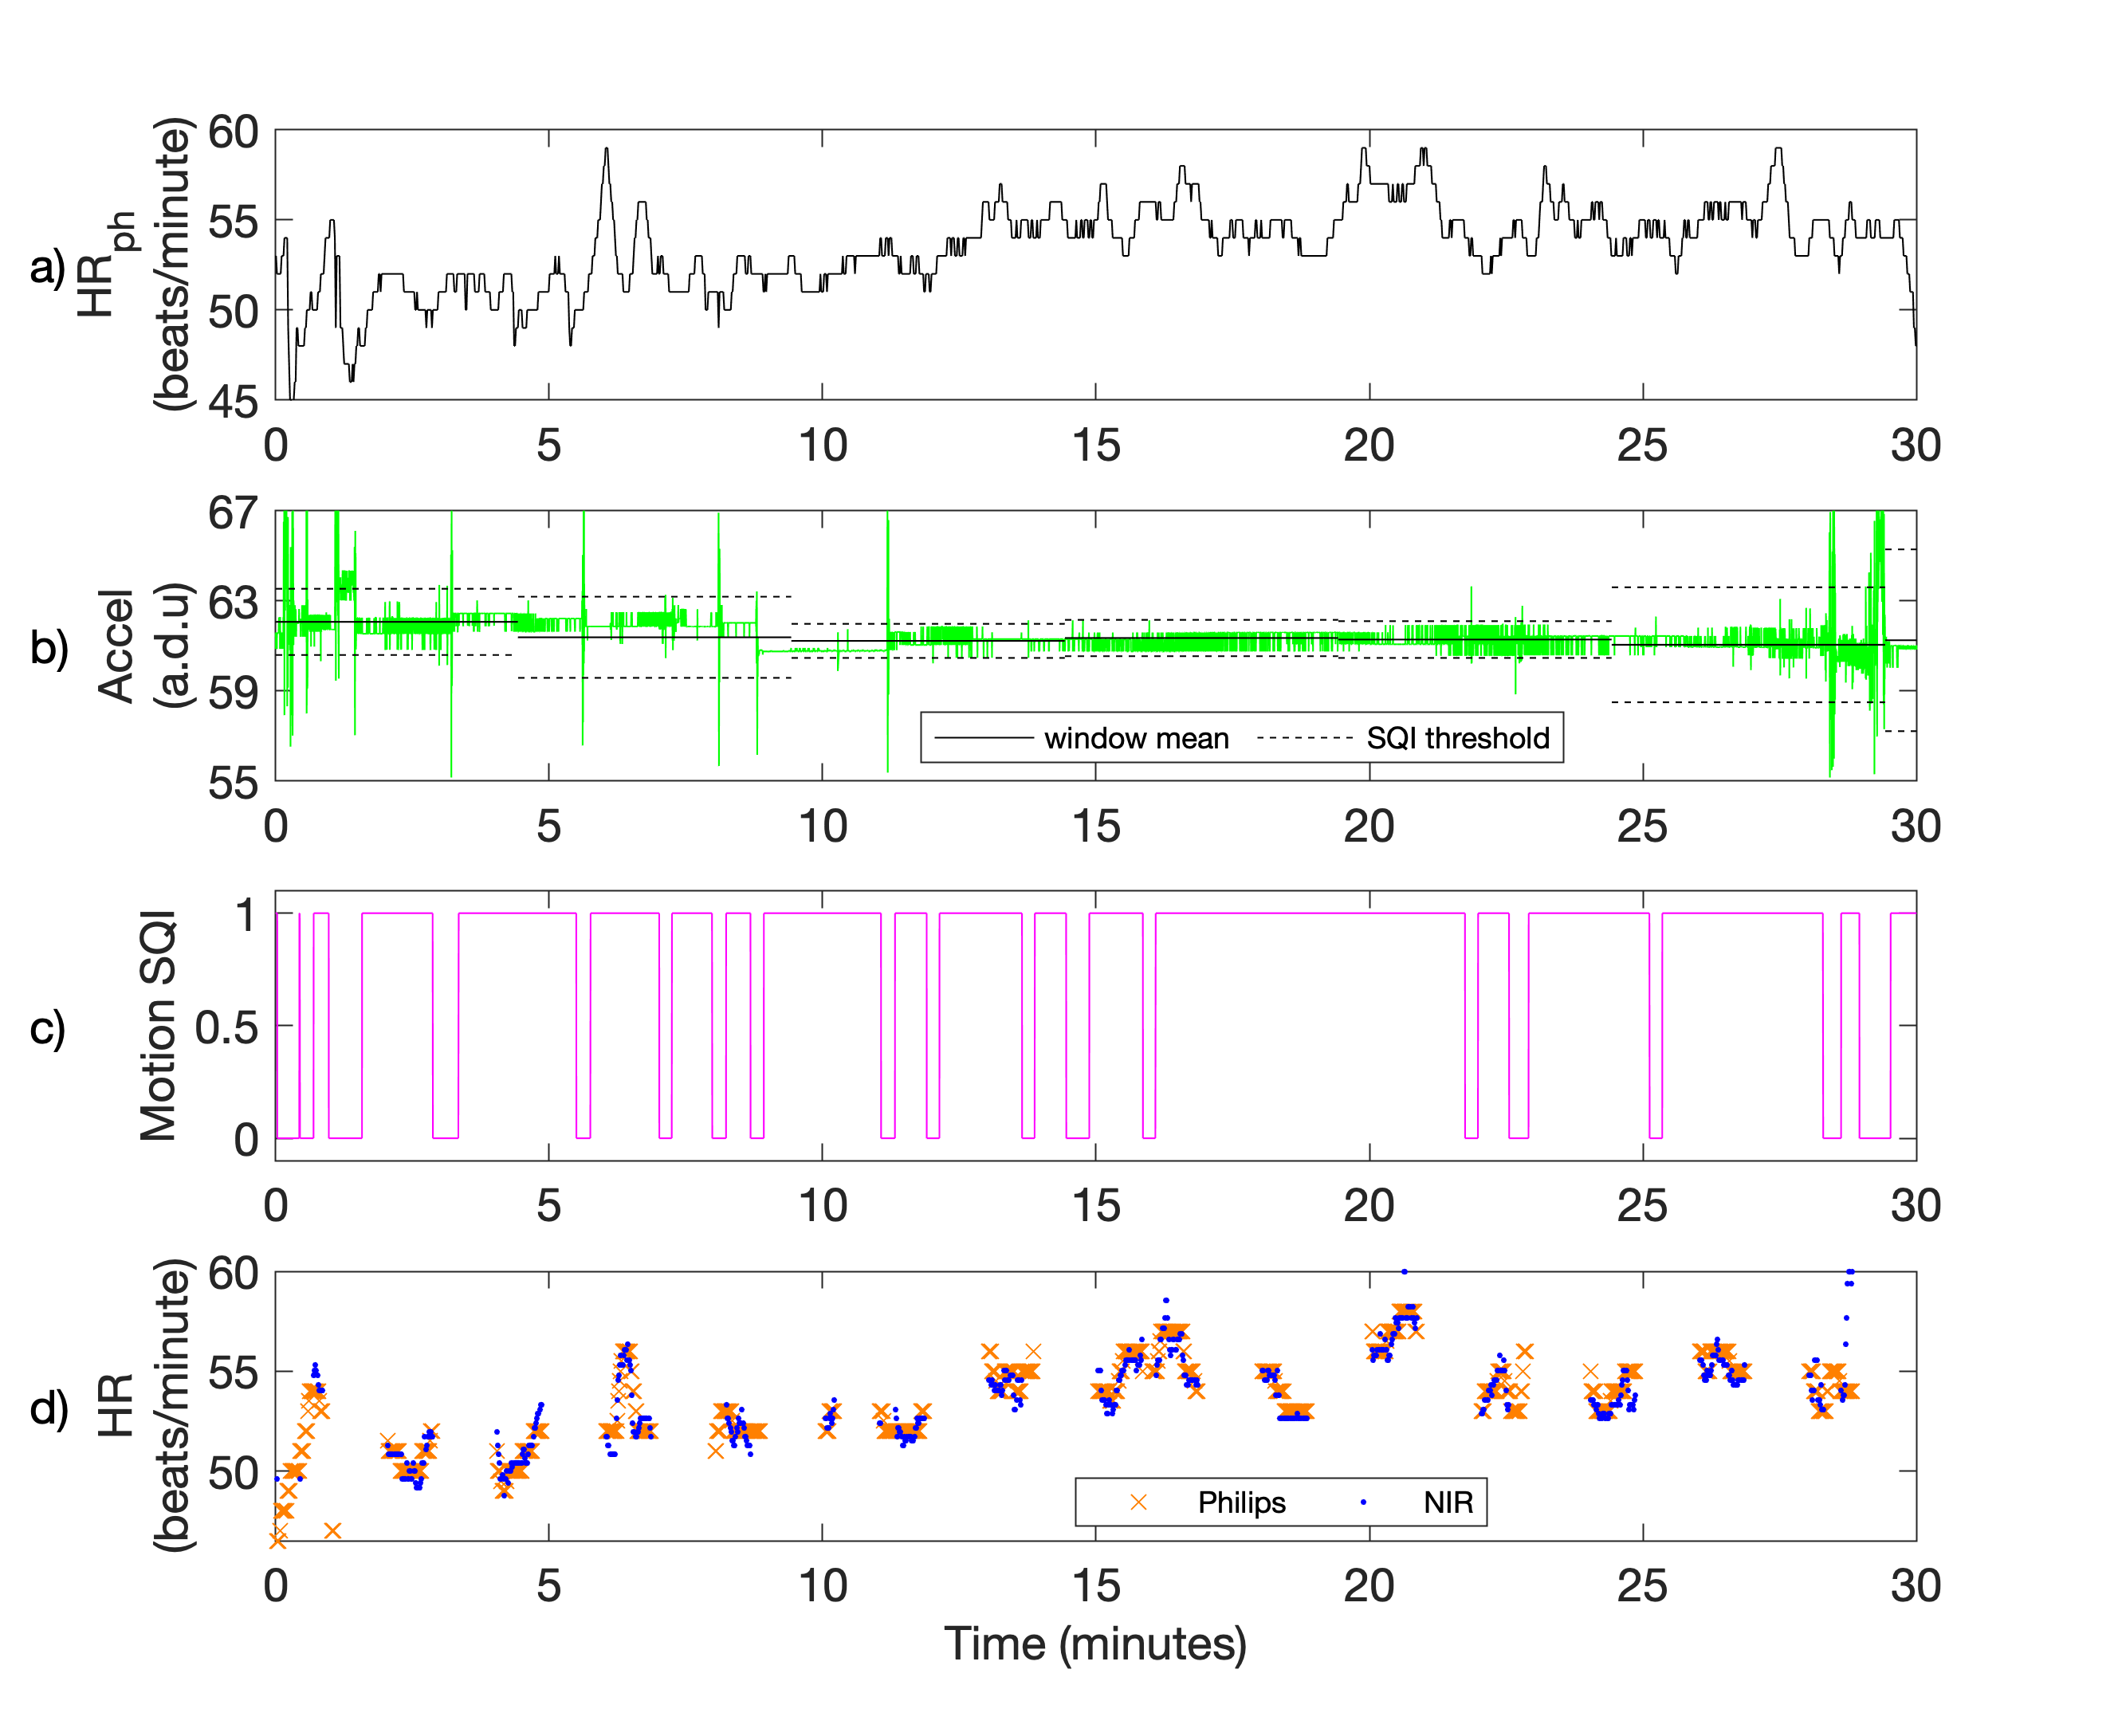
\includegraphics[width = 12 cm]{./figures/HR_Series_003.png}
    \caption[Comparison between HR provided by the Philips monitor and the HR estimates computed by the proposed algorithms.]{Comparison between HR provided by the Philips monitor and the HR estimates computed by the proposed algorithms. a) HR from Philips monitor. b) Accelerometer data recorded by the Wavelet Health device. c) Motion \gls{sqi}. Values of 1 correspond to periods of good-quality signal; Conversely values of 0 correspond to periods of poor quality signal. d) Estimated HR from NIR signal compared to reference HR.}
    \label{HRseries}
    \end{figure}

 
 \begin{table}
\centering
\caption{Summary of results for the proposed algorithms to estimate \gls{hr} from the NIR signals for the 10 patients analysed.}
\label{metrics}
\vspace{2em}
\begin{tabular}{p{2cm} r r r r}
 \tableHeaderStart 
Patient Number & MAE* & MAD* & RMSE* & r \\
   	 \midrule
      001 & 0.6  & 0.6 & 0.9 & 0.92 \\        
      002 & 1.6 & 1.6 & 2.0 & 0.94 \\   
      003 & 0.6  & 0.6   & 0.8 & 0.99\\        
      004 & 1.0 & 1.0  & 1.3  & 0.98\\   
      005 & 0.7 & 0.7 & 1.0 & 0.98  \\  
      006 & 1.9 & 1.9 & 2.9 & 0.89 \\          
      007 & 1.2 & 1.2  & 1.8  & 0.97 \\   
      008 & 2.3 & 2.2 & 3.1 & 0.9 \\   
      009 & 0.7 & 0.7 & 1.0 & 0.96\\   
      010 & 1.2 & 1.2 & 1.5 & 0.97 \\   
      \midrule        
      Overall & 1.2 & 1.2 & 1.8 & 0.99 \\
 \tableHeaderEnd
      \multicolumn{4}{l}{*Values in beats/minute}     
       \end{tabular}
\end{table}

Figure \ref{hrsummary} (a) shows the Bland- Altman plot comparing the Philips and estimated heart rate values for all 10 patients. The plot shows a mean bias of 0.16 beats/min, 95\% of the differences fall within [-3.4, 3.1] beats/min, the correlation coefficient is 0.99. The MAE between both heart rate measurements was 1.2 beats/min with a MAD of 1.2 beats/min. 
 

\begin{figure}
    \centering
\includegraphics[width = 12 cm]{./figures/HR_summary_plot_{IR}_1.png}
 \caption[Comparison between the reference and estimated heart rate for the 10 patients analysed.]{Comparison between the reference and estimated heart rate for the 10 patients analysed. a) Bland-Altman plot, b) histogram of the differences between the two heart rate estimates. c) Correlation plot showing a positive correlation between the two measurements, the red line represents the linear fit.}
 \label{hrsummary}
\end{figure}


\subsection{Respiratory rate}

Figure~\ref{RRseries} shows a comparison between the reference RR from the Philips monitor and the estimated RR computed from the Wavelet Health device by the proposed algoithms. Table \ref{RRmetrics3} shows \gls{mae}, \gls{mad} and \gls{rmse} values, correlation values and the error distribution computed across 10 subjects in the dataset. 
 

\begin{figure}
	\centering
	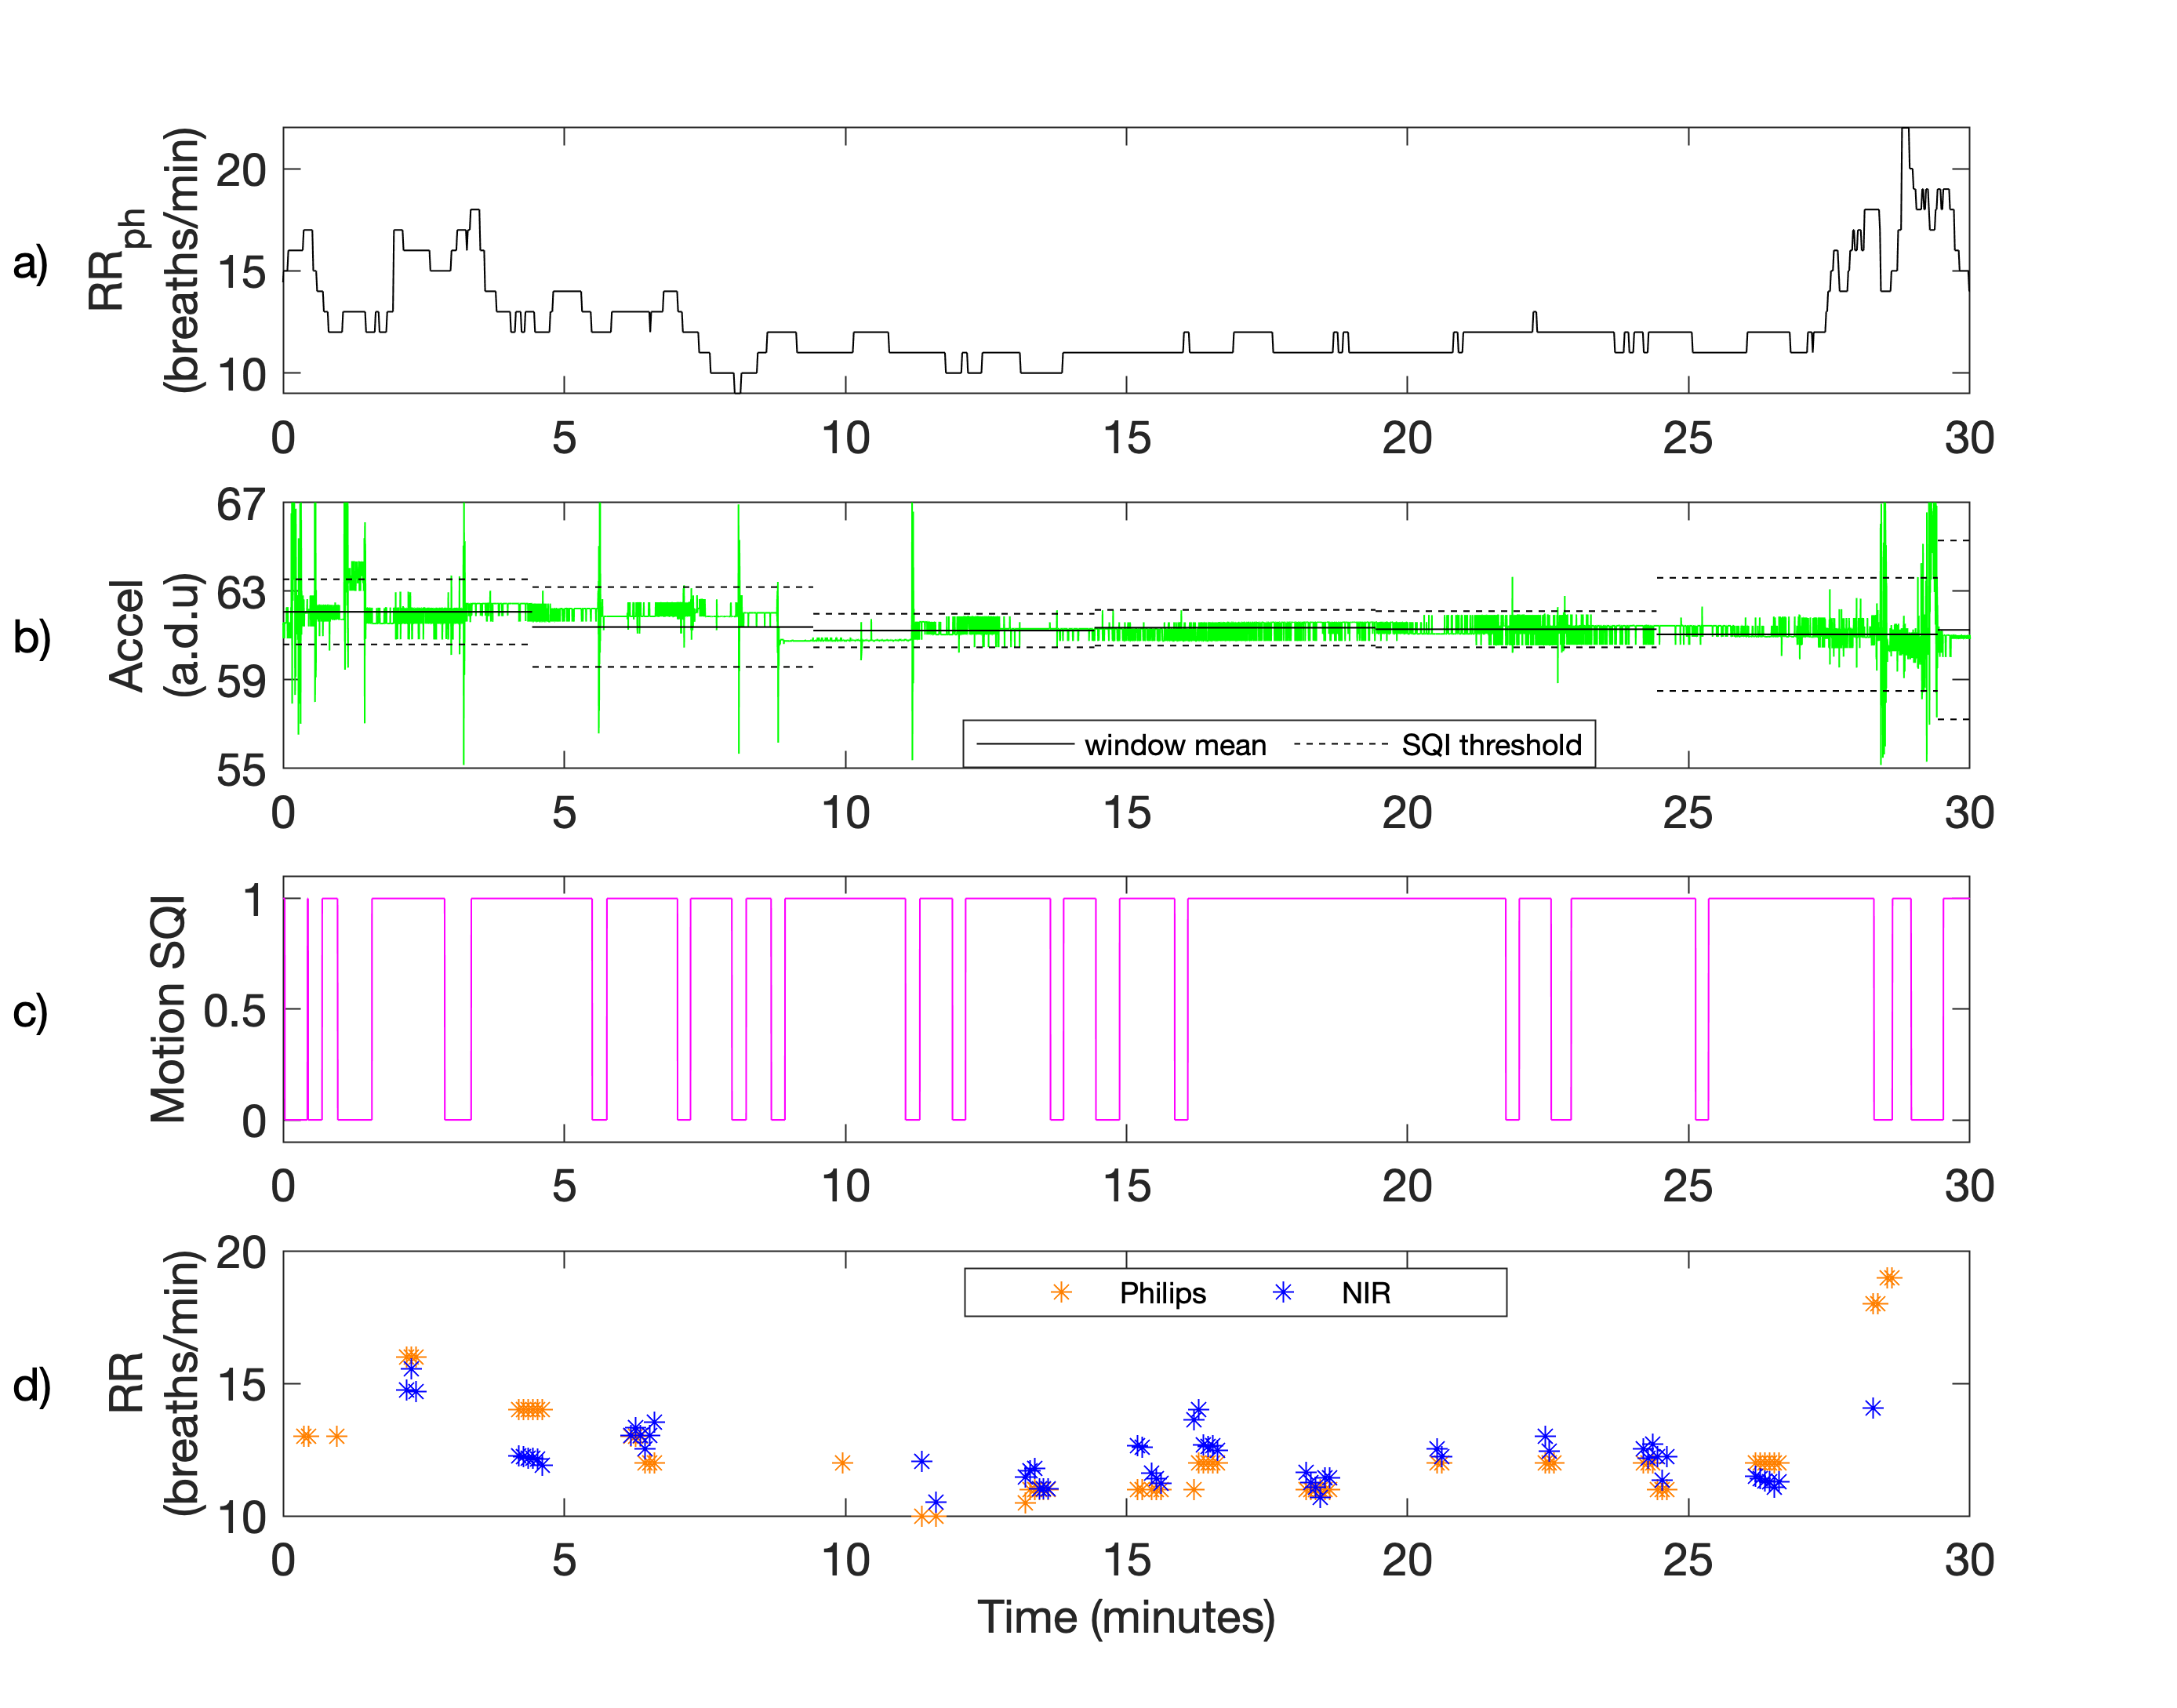
\includegraphics[width=0.9\linewidth,keepaspectratio=true]{RRmethALL_Series_003.png}
	 \caption[Comparison between the reference respiratory rate provided by the Philips monitor and the estimated respiratory rates.]{Comparison between the reference RR provided by the Philips monitor and the estimated respiratory rates a) RR from Philips monitor; b) Acceleration data from the Wavelet Health device; c) Motion \gls{sqi}. Values of 1 correspond to periods of good-quality signal; Conversely values of 0 correspond to periods of poor quality signal; d) RR medians computed from reference respiratory rate and computed respiratory rate from the NIR signal.}
	 \label{RRseries}
\end{figure}
    
    
    
\begin{table}
	\centering
	\caption[PLEASE COMPLETE ME MYA]
	{
		Summary of the results for the proposed algorithms to estimate respiratory rate.
	}
	\begin{tabular}{p{0.8 cm} | r r r r| r r r r| r r r r }
		 \tableHeaderStart 
		&  \multicolumn{4}{|c|}{Amplitude modulation} & \multicolumn{4}{|c|}{Frequency Modulation}  & \multicolumn{4}{|c}{Combined Method} \\
		Patient No.&MAE*&MAD*&RMSE*&r&MAE*&MAD*&RMSE*&r&MAE*&MAD*&RMSE*& r\\
		   	 \midrule
		      001  & 1.4 & 1.4 & 2.0 & 0.33 & 1.4 & 1.4 & 2.0 & 0.60 & 0.9 & 0.9 & 1.2 & 0.61 \\        
		      002 & 2.7 & 2.0 & 3.6 & 0.45  & 2.2 & 1.9 & 2.9 & 0.54 & 1.7 & 1.3 & 2.2 & 0.74\\   
		      003 &  2.5 & 2.2 & 3.5 & 0.27 & 3.0 & 2.8 & 4.5 & 0.09 & 1.0 & 1.0 & 1.5 & 0.79\\        
		      004 & 1.9 & 1.8 & 2.5 & 0.19 & 1.4 & 1.4 & 1.9 & 0.51 & 1.5 & 1.4 & 2.0 & 0.42\\   
		      005 & 1.4 & 1.3 & 1.7 & 0.55 & 2.4 & 1.8 & 3.0 & 0.53 & 1.4 & 1.2 & 1.8 & 0.57\\  
		      006 & 4.0 & 2.9 & 5.0 & - 0.32 & 2.3 & 2.0 & 3.0 & 0.06 & 2.5 & 2.4 & 3.6 & -0.17\\          
		      007 & 3.7 & 2.8 & 4.5 & -0.05 & 1.8 & 1.8 & 2.5 & 0.08 & 2.0 & 2.0  & 2.5 & 0.11\\   
		      008  & 3.6 & 2.2 & 4.6 & 0.08 & 4.4 & 2.7 & 5.3 & 0.17 & 3.4 & 2.0 & 4.1 & 0.19 \\   
		      009 & 1.4 & 1.2 & 1.8 & 0.36 & 4.2 & 3.7 & 5.6 & -0.16 & 0.8 & 0.8 & 1.0 & 0.46\\   
		      010 & 2.6 & 3.2 & 4.2 & 0.34 & 1.2 & 1.3 & 3.3 & -0.09 & 0.6 & 0.6 & 0.8 & 0.89\\   
		      \midrule        
		      Overall & 2.5 & 2.5 & 3.5 & 0.52 & 2.3 & 2.3 & 3.5 & 0.47 & 1.6 & 1.6 & 2.3 & 0.74\\
		      \tableHeaderEnd
		      \multicolumn{12}{l}{*Values in breaths/minute}
	\end{tabular}
	\label{RRmetrics3}
\end{table}    
    
Figure \ref{RRsummary3}(a) shows the Bland- Altman plot comparing the Philips and estimated respiratory rate values for all 10 patients. The plot shows a mean bias of 0.18 breaths/min, most of the differences falling within [-4.3, 4.6] breaths/min, the correlation coefficient is 0.74. The MAE between both respiratory rate measurements was 1.6 breaths/min with a MAD of 1.6 breaths/min. 

\begin{figure}
    \centering
	\includegraphics[width = 11 cm]{./figures/RR_summary_plot_method_ALL1.png}
	 \caption[Comparison between the reference and estimated RR for the 10 patients in the dataset.]{Comparison between the reference and estimated RR for the 10 patients in the dataset. a) Bland-Altman plot; b) histogram of the differences between the two \gls{rr} estimates; c) Correlation plot shows a positive correlation between the two measurements, the red line represents the linear fit.}
	 \label{RRsummary3} 
\end{figure}

\subsection{$SpO_2$}


Figure~\ref{spo2series} shows the relationship between the ratio of ratios computed using the Red/NIR signals from the Wavelet Health wearable device, compared with the reference  \gls{$SpO_{2}$} provided by the Philips monitor for a sample recorded session. An inverse correlation between \gls{$SpO_{2}$} and the Red/NIR ratio can be seen.
Figure~\ref{spo2_scatter} shows the scatter plots comparing the red/NIR ratio obtained from the Wavelet Health to the Philips \gls{$SpO_{2}$}  values for all 10 patients. The plots shows correlation coefficient  ranging from r = 0.62 to r = 0.98.


\begin{figure}
\centering
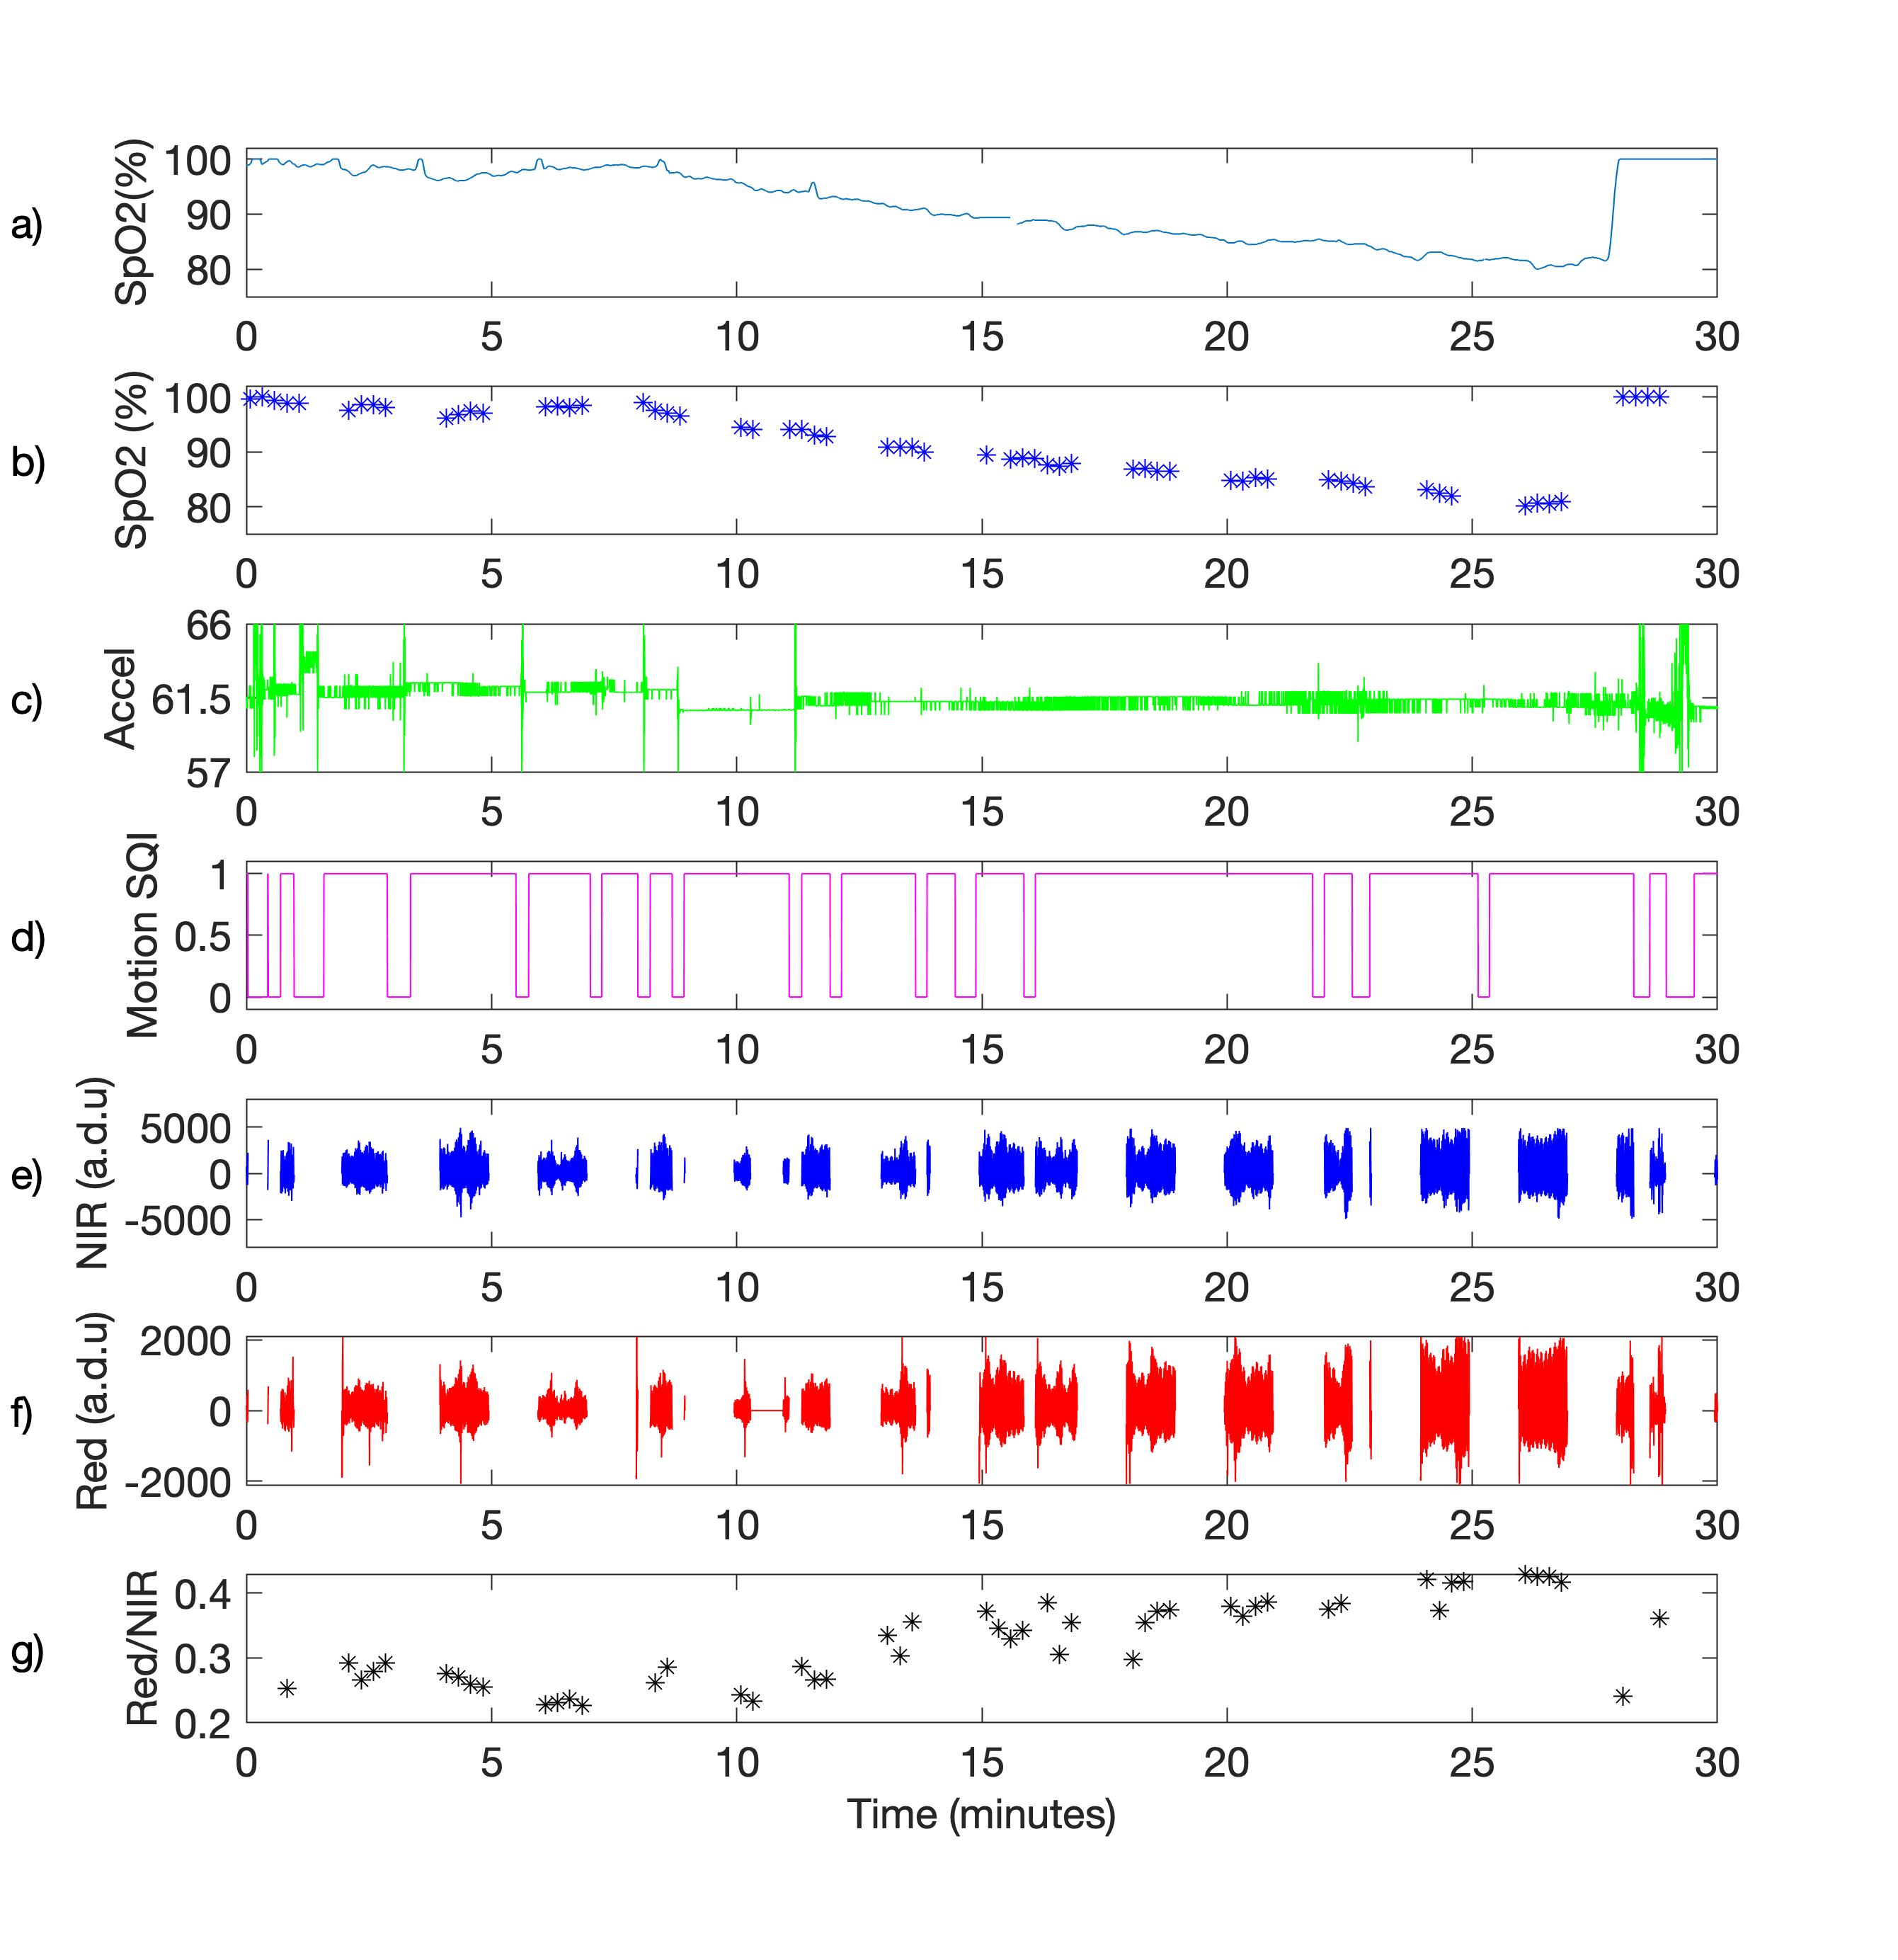
\includegraphics[width = 11 cm]{./figures/SpO2_Series_003.png}
    \caption[Comparison of the trend between the Red/NIR ratio and the reference \gls{$SpO_{2}$}.]{Comparison of the trend between the Red/NIR ratio and the reference \gls{$SpO_{2}$}. a) Reference \gls{$SpO_{2}$}; b) Medians of the reference\gls{$SpO_{2}$}; c) Accelerometer data; d) Motion SQI;  e) NIR signal amplitudes; f) Red signal amplitudes; g) Red/NIR amplitudes ratio.} \label{spo2series}
\end{figure}



\begin{figure}
    \centering
\includegraphics[width = 10 cm]{./figures/scatter_plot_1.png}
    \caption[Correlation plots of the Red/NIR Ratio for the 10 patients in the dataset.]{Correlation plots of the Red/NIR Ratio for the 10 patients in the dataset. Increased red light absorbance (increased Ratio) is associated with increased de-oxyhaemoglobin, i.e., lower \gls{$SpO_{2}$}. The red line represents the linear fit.}
    \label{spo2_scatter} 
\end{figure}


\section{Discussion}

Heart rate is a vital sign that can be estimated from a wearable device, which makes it a good candidate for validating the proposed signal processing algorithms. As can be seen in figure \ref{hrsummary} and table \ref{metrics}, our HR estimates are comparable to the values computed by a reference medical device. The mean bias of 0.16 beats/min and correlation coefficient of 0.99 suggests that our proposed signal processing algorithms work adequately.

Respiratory rate is considerably more difficult to estimate from a wearable device. The lower correlation coefficient (r = 0.74) and errors (MAE and MAD of 1.6 breaths/min) shown in figure \ref{RRsummary3} and table \ref{RRmetrics3} respectively, are clear indication of this. By combining the two proposed methods using an additional SQI (respiratory difference) the estimation results were improved and there was a low bias and positive correlation present. 

The Wavelet Health device is a novel wrist worn device. Comparisons between \gls{$SpO_{2}$} from the Philips monitor and Wavelet Health device showed inconsistent performance showing that the device is not adequate to estimate \gls{$SpO_{2}$} during desaturation periods.

\section{Conclusion}

This chapter presented the algorithms for estimating vital signs (\gls{hr},\gls{rr} and \gls{$SpO_{2}$}) from the Wavelet Health wearable device. The \gls{hr} results had minimal errors with a positive correlation coefficient of 0.99. The other results (\gls{rr} and \gls{$SpO_{2}$}) had errors greater than the WHO guidelines. New and improved methods are needed to design technologies that can estimate vital signs for the target population of this report
